% ============================================================================
% paper_espanol.tex  --  Versión en español. Texto en paper/espanol/; tablas en
% tables/es/ y figuras en figures/es/, generadas por scripts/R/09_tables.R y
% save_fig(). Está en la raíz del repositorio para que todas las rutas
% funcionen igual en local y en Overleaf, donde BibTeX corre desde la raíz.
%   pdflatex paper_espanol ; bibtex paper_espanol ; pdflatex x2   (o tectonic)
% ============================================================================
\documentclass[12pt]{article}

\usepackage[utf8]{inputenc}
\usepackage[T1]{fontenc}
\usepackage{lmodern}
\usepackage[spanish,es-noshorthands,es-nodecimaldot]{babel}
\usepackage{amsmath,amssymb,amsthm}
\usepackage{graphicx}
\usepackage{booktabs}
\usepackage{threeparttable}
\usepackage{caption}
\usepackage{subcaption}
\usepackage{float}
\usepackage[margin=1in]{geometry}
\usepackage{setspace}
\usepackage[authoryear,round]{natbib}
\bibliographystyle{paper/espanol/apalike-es}
\usepackage[hidelinks]{hyperref}
\usepackage{xcolor}
\usepackage{siunitx}
\usepackage{enumitem}

\captionsetup{font=small,labelfont=bf}
\setlength{\parskip}{2pt}
\graphicspath{{figures/es/}}

\newcommand{\Low}{\mathrm{Low}}
\newcommand{\Post}{\mathrm{Post}}

\title{\textbf{Exposición diferencial a un salario mínimo nacional: salarios, contratación formal e informalidad en el Perú} \thanks{Este documento utiliza los módulos trimestrales de empleo de uso público de la Encuesta Nacional de Hogares (ENAHO) del Instituto Nacional de Estadística e Informática (INEI). Todas las estimaciones usan los factores de expansión de la encuesta; el paquete de replicación está disponible en el repositorio que acompaña al documento. Cualquier error es responsabilidad exclusiva del autor.}}

\author{Eric Torres Ramirez\\
  \small Pontificia Universidad Católica del Perú\\
  \small \texttt{etorresram@gmail.com}}
\date{\textbf{Borrador}\\ Esta versión: \today}

\begin{document}
\maketitle

\begin{abstract}
\noindent En mayo de 2022 el Perú elevó su salario mínimo nacional en 10 por ciento, rompiendo la barrera de los mil soles. Como el mínimo es único a nivel nacional, identifico sus efectos comparando a los trabajadores de baja educación, la mayoría de los cuales ganaban menos que el nuevo mínimo, con los de mayor educación, con datos trimestrales de la ENAHO para 2021-2024. La reforma no elevó los salarios relativos de los trabajadores de baja educación. Los empleadores formales ajustaron los salarios al nuevo mínimo; sin embargo, solo el 13\% de los trabajadores de baja educación tiene un empleo formal. Lo que sí cambió fue dónde trabajan, su empleo formal cayó 4.6 puntos porcentuales, un quinto de su nivel inicial, y el trabajo independiente aumentó 3.6 puntos. Un análisis complementario de panel muestra que el ajuste no vino de despidos, sino de menos ingresos al empleo formal; es decir, la tasa a la que los trabajadores informales pasaban a la formalidad cayó casi a la mitad. Repetí el análisis principal para el aumento de igual magnitud de 2025, en un mercado laboral más estable, y no encuentro un desplazamiento comparable. En suma, donde la informalidad es amplia, subir el salario mínimo reordena el empleo más de lo que eleva los salarios relativos.

\medskip
\noindent\textbf{Palabras clave:} salario mínimo; informalidad; educación; diferencias en diferencias; Perú.\\
\noindent\textbf{Códigos JEL:} J23, J31, J38, J46, O17.
\end{abstract}

\newpage
\setstretch{1.15}

\section{Introducción}\label{sec:intro}

Que un salario mínimo beneficie a los trabajadores a quienes se dirige depende de a cuántos de ellos llega realmente. En los países en desarrollo, una gran parte del empleo queda fuera del alcance de la regulación laboral, de modo que un piso salarial legal puede elevar la remuneración de los trabajadores cubiertos, desplazar a algunos de ellos hacia el sector informal no cubierto o funcionar solo como un punto de referencia para salarios que las empresas formales habrían pagado de todos modos. Cuál de estas fuerzas predomina es una pregunta empírica, y su respuesta depende de cuán vinculante es el piso, de qué tan bien se fiscaliza y de con cuánta libertad se mueven los trabajadores entre los márgenes formal e informal. Estudio estas preguntas para el Perú, un país que combina un salario mínimo elevado en relación con la remuneración mediana con una de las tasas de informalidad laboral más altas de América Latina.

Aprovecho el aumento del salario mínimo nacional del Perú (la \emph{Remuneración Mínima Vital}, o RMV) de 930 a 1025 soles, dispuesto por el Decreto Supremo 003-2022-TR y vigente desde el 1 de mayo de 2022. Este aumento nominal de 10.2 por ciento fue el primer cambio de la RMV en cuatro años y se produjo cuando el mercado laboral salía de la pandemia. Un hecho institucional central determina el análisis: el Perú fija un único salario mínimo nacional, sin variación regional ni sectorial en el régimen general. Por lo tanto, no existe variación transversal en el nivel de la política ni una adopción escalonada que aprovechar. Como señala \citet{jimenez_2023} para la reforma de 2016, una identificación creíble debe provenir, en cambio, de una \emph{exposición} diferenciada a una política que cambia para todos al mismo tiempo.

Mi fuente de exposición diferenciada es la educación. En los trimestres previos a la reforma, el salario mensual equivalente mediano de un asalariado privado de baja educación era de 950 soles, casi exactamente el mínimo anterior de 930, y el 57 por ciento de los asalariados de baja educación percibía menos que el \emph{nuevo} piso de 1025 soles en vísperas de la reforma; un aumento de diez por ciento en ese piso resulta, por ello, muy vinculante para este grupo. Los trabajadores de alta educación, en cambio, tienen un salario mediano muy por encima del mínimo y es menos probable que este los alcance, aunque una minoría considerable sigue expuesta a través del trabajo informal o por cuenta propia. Esta brecha de exposición, y no el supuesto de una exposición nula del grupo de comparación, motiva un diseño de diferencias en diferencias que contrasta a los trabajadores de baja educación (aquellos con, a lo sumo, secundaria completa, cerca de dos tercios de la población en edad de trabajar) con los trabajadores de alta educación (aquellos con cualquier nivel de educación superior). El diseño traslada una larga tradición de medición de los efectos del salario mínimo a partir de la variación en la incidencia (\emph{bite}) de la política entre grupos o regiones \citep{card_1992, lee_1999, machin_manning_rahman_2003} a un contexto con una sola reforma nacional y datos de hogares trimestrales y ricos en información.

Utilizo los módulos trimestrales de empleo de uso público de la Encuesta Nacional de Hogares (ENAHO) desde 2021Q1 hasta 2024Q4, que rodean la reforma con cinco trimestres previos y diez trimestres posteriores limpios; el trimestre de transición 2022Q2, en el que la reforma entró en vigor a mitad de trimestre, se excluye de la especificación base y se reincorpora en una prueba de robustez. Los datos son cortes transversales repetidos, y su frecuencia trimestral me permite estimar un estudio de eventos dinámico, contrastar tendencias previas diferenciadas por educación y seguir el efecto durante más de dos años después de la reforma. Examino un conjunto amplio de resultados: salarios reales por hora e ingresos mensuales, la probabilidad de estar empleado y de participar en la fuerza laboral, la incidencia del empleo formal frente al informal, las horas de trabajo y la división del empleo entre trabajo asalariado y trabajo independiente. En todo el análisis pondero con los factores de expansión y agrupo la inferencia por departamento; y como el tratamiento se asigna a un nivel agregado, complemento los errores estándar robustos por conglomerados convencionales con la corrección para muestras pequeñas de \citet{pustejovsky_tipton_2018} y con inferencia por aleatorización.

Surgen tres resultados. Primero, y de manera más robusta, la reforma desplazó la \emph{composición} del empleo de baja educación lejos del trabajo asalariado formal. La probabilidad de que un trabajador de baja educación tenga un empleo formal cae en 4.6 puntos porcentuales, cerca de una quinta parte de la tasa base de formalidad del grupo, de 23 por ciento, y el trabajo independiente aumenta en 3.6 puntos. Las tendencias previas de formalidad de estas estimaciones superan su prueba conjunta, con una pequeña deriva residual que cuantifico y corrijo; los efectos aparecen inmediatamente después de la reforma y persisten, son mayores en los departamentos donde el nuevo piso corta más profundamente la distribución salarial y los confirma un diseño independiente de exposición continua que relaciona los resultados con el índice de Kaitz regional previo a la reforma y admite inferencia por aleatorización basada en el diseño. Las personas enlazadas del Panel ENAHO 2020--2024 revelan el flujo que subyace al stock: los trabajadores formales en su puesto fueron retenidos, mientras que la tasa a la que los trabajadores informales de baja educación ingresaban a empleos formales cayó casi a la mitad, de modo que la reasignación operó mediante la creación de vínculos formales y no mediante su destrucción. Segundo, no hay evidencia de que la reforma elevara la remuneración del grupo, pero no porque el piso sea letra muerta. Dentro del sector formal, donde opera la fiscalización, el pico de ingresos en el mínimo anterior se traslada casi por completo al nuevo, y cae la proporción de asalariados formales que perciben menos que el nuevo piso; entre los asalariados informales esa proporción \emph{aumenta}, y como solo el 13 por ciento de los trabajadores ocupados de baja educación son formales, ambas respuestas se compensan: la proporción agregada por debajo del piso no se mueve, ningún decil de la distribución salarial muestra una ganancia y el efecto estimado sobre el logaritmo del salario real por hora promedio es negativo y no significativo. La conclusión de que no hubo una elevación salarial descansa en la evidencia de cumplimiento y distributiva, cuyos diagnósticos son limpios; la regresión del salario promedio, en sí misma, presenta una prueba de tendencias previas rechazada, impulsada por un único trimestre de inicios de 2021, y soy explícito sobre lo que puede y no puede descartar. Tercero, la tasa de empleo de los trabajadores de baja educación cae en 2.5 puntos porcentuales, pero este margen es el menos robusto: no supera las pruebas placebo en el tiempo, presenta una clara tendencia previa diferenciada asociada a la recuperación de la pandemia y no escala con la exposición regional, por lo que no le doy una interpretación causal. En todo el análisis acoto las conclusiones con el análisis de sensibilidad de \citet{rambachan_roth_2023} y con una batería de pruebas de especificación y placebo. Luego replico el diseño completo en la reforma de enero de 2025, que elevó la RMV a 1130 soles en un período más tranquilo, posterior a la pandemia: allí tampoco aparece respuesta salarial, ni tampoco la reasignación, lo que interpreto como evidencia de que el margen en el que el salario mínimo resulta vinculante depende del estado del mercado laboral.

La contribución es una combinación y no una herramienta nueva, y la planteo sin exagerarla. Hasta donde sé, esta es la primera evaluación de la reforma del salario mínimo peruano de 2022 y el primer estudio de cualquier reforma peruana que utiliza la ENAHO trimestral posterior a la pandemia; la evidencia microeconómica existente se detiene en la reforma de 2016 \citep{jimenez_2023} o en las reformas de inicios de la década de 2000 \citep{jaramillo_lopez_2006, cespedes_2005}. Es también el primero en hacer de la heterogeneidad por educación el objeto central de un estudio de eventos a nivel de trabajador sobre el salario mínimo peruano, mientras que los trabajos previos analizan la heterogeneidad por rango de ingresos o edad, o construyen una dosis de exposición a nivel departamental. Es también, hasta donde sé, el primero en usar el Panel ENAHO enlazado para medir transiciones de formalidad a nivel de trabajador en torno a una reforma del salario mínimo peruano, lo que me permite separar la retención de los trabajadores en su puesto de la entrada de nuevos trabajadores a empleos formales. Y sitúa el margen informal en el centro del análisis, al mostrar que el ajuste opera a través de la composición del empleo y no de la remuneración. No reclamo novedad para la idea de identificación, que es el diseño estándar de exposición o de incidencia, ni para las herramientas econométricas; el valor agregado es la combinación de una reforma nueva y un período posterior a la pandemia relevante para la política pública con un diseño a nivel de trabajador basado en la educación y un tratamiento cuidadoso de la informalidad y de las amenazas a la identificación que tal diseño implica.

El resto del artículo se organiza como sigue. La Sección~\ref{sec:institutional} describe el salario mínimo peruano y la reforma, y la Sección~\ref{sec:literature} sitúa el artículo en la literatura. La Sección~\ref{sec:data} presenta los datos y la construcción de las variables clave, y la Sección~\ref{sec:strategy} expone la estrategia empírica y los supuestos de identificación. La Sección~\ref{sec:results} reporta los resultados principales, la Sección~\ref{sec:robustness} las pruebas de robustez e inferencia y la Sección~\ref{sec:heterogeneity} el análisis de heterogeneidad y distributivo. La Sección~\ref{sec:discussion} discute los mecanismos, la validez externa y las limitaciones, y la Sección~\ref{sec:conclusion} concluye.

\section{Contexto institucional}\label{sec:institutional}

\subsection{El salario mínimo peruano}

El Perú fija un único salario mínimo nacional, la \emph{Remuneración Mínima Vital} (RMV), que se aplica a los trabajadores del régimen laboral de la actividad privada. A diferencia de sistemas federales como los de Estados Unidos o Brasil, y de los países con pisos salariales por ocupación o por región, el Perú no tiene un mínimo legal subnacional ni específico por industria en el régimen general. Un pequeño número de regímenes especiales está indexado a la RMV: la minería tiene una bonificación legal sobre ella, el régimen agrario de la Ley 31110 fija una remuneración diaria anclada en ella y el régimen de la micro y pequeña empresa (MYPE) aplica el mismo piso. Ninguno de ellos introduce variación transversal en el nivel de la política.\footnote{Como el régimen agrario paga una remuneración diaria bajo reglas propias, identifico la agricultura en todo el análisis y muestro la robustez de los resultados a su exclusión (Sección~\ref{sec:robustness}).} La consecuencia para el diseño de investigación es decisiva: como el nivel de la RMV es común a todo el país, no existe variación transversal en la política ni un calendario escalonado de adopción. Cualquier diseño de investigación creíble debe, por tanto, aprovechar las diferencias en el grado de exposición de los trabajadores a un cambio que llega a todos al mismo tiempo.

En principio, la RMV debe ser ajustada periódicamente por el Consejo Nacional de Trabajo, de carácter tripartito, en función de la inflación y la productividad. En la práctica, el Consejo nunca ha fijado la RMV, y su nivel lo determina discrecionalmente el Poder Ejecutivo mediante un Decreto Supremo. En consecuencia, los ajustes son poco frecuentes e irregulares tanto en su calendario como en su magnitud, y el Perú figura entre los países de la región que fijan su salario mínimo de forma más volátil \citep{jimenez_2023, cespedes_2005}. La RMV se había mantenido en 930 soles desde abril de 2018.\footnote{Fijada por el Decreto Supremo 004-2018-TR. Los dos aumentos anteriores elevaron la RMV de 750 a 850 soles en mayo de 2016 y de 850 a 930 soles en abril de 2018, de modo que la reforma de 2022 siguió a un congelamiento inusualmente largo.}

Dos características hacen que la RMV sea inusualmente vinculante para los estándares internacionales. Primero, su relación con el salario mediano es alta. En mi muestra previa a la reforma, el salario mensual equivalente mediano nacional de un asalariado privado es de 1000 soles, de modo que el mínimo anterior de 930 equivalía al 93 por ciento de la mediana, el nuevo mínimo quedó ligeramente por encima de ella, y el índice de Kaitz, la razón entre el mínimo y el salario mediano, es cercano a uno a nivel nacional y se aproxima a dos en los departamentos más pobres. Segundo, el cumplimiento dista de ser universal. En línea con trabajos anteriores \citep{jaramillo_lopez_2006, cespedes_2005}, una gran proporción de trabajadores percibe menos que el piso legal, especialmente en las zonas rurales, en las empresas pequeñas y en el sector informal, mientras que el cumplimiento dentro de las empresas formales registradas es alto. La capacidad de fiscalización es limitada.\footnote{La inspección laboral está a cargo de la Superintendencia Nacional de Fiscalización Laboral (SUNAFIL), cuyo personal inspector es escaso fuera de Lima. Trabajos anteriores estiman el incumplimiento total de la RMV en alrededor de 30 a 40 por ciento, concentrado en las zonas rurales, las empresas pequeñas y el sector informal \citep{jaramillo_lopez_2006, cespedes_2005}.} Estas características implican que un aumento nominal de la RMV puede ser mecánicamente vinculante para los trabajadores formales cercanos al piso y, a la vez, dejar a buena parte del sector informal sin cobertura formal, de modo que el alcance real de la política depende del grado de informalidad y de la facilidad de movimiento entre los márgenes formal e informal.

\subsection{La reforma de 2022}

La reforma que estudio fue dispuesta por el Decreto Supremo 003-2022-TR, publicado el 3 de abril de 2022, y entró en vigor el 1 de mayo de 2022. Elevó la RMV de 930 a 1025 soles, un aumento de 95 soles o 10.2 por ciento, el primer cambio en cuatro años. La Figura~\ref{fig:mw} muestra el valor nominal y real de la RMV durante 2021--2025. Conviene destacar dos puntos. El aumento nominal de 10.2 por ciento fue compensado en parte por la inflación, que rondó el 8 por ciento durante 2022, de modo que el aumento del valor real del piso fue más modesto y se erosionó en los dos años siguientes. Esto modera el tamaño esperado de cualquier respuesta salarial y es relevante al comparar mis estimaciones con las de episodios de menor inflación. La reforma ocurrió, además, durante la recuperación posterior a la pandemia, un período de turbulencia inusual en el mercado laboral que abordo de forma explícita en el análisis empírico.

Una segunda reforma, dispuesta por el Decreto Supremo 006-2024-TR y vigente desde el 1 de enero de 2025, elevó la RMV a 1130 soles. Este cambio queda justo fuera de mi ventana principal de estudio, pero los trimestres de la ENAHO de 2025 están disponibles y utilizo esta segunda reforma como una réplica fuera de muestra del diseño en la Sección~\ref{sec:robustness}. Ambas reformas son de magnitud muy similar, 10.2 por ciento cada una, lo que convierte al episodio de 2025 en un ejercicio natural de validación en un entorno más tranquilo, posterior a la pandemia.

\begin{figure}[!t]
\centering
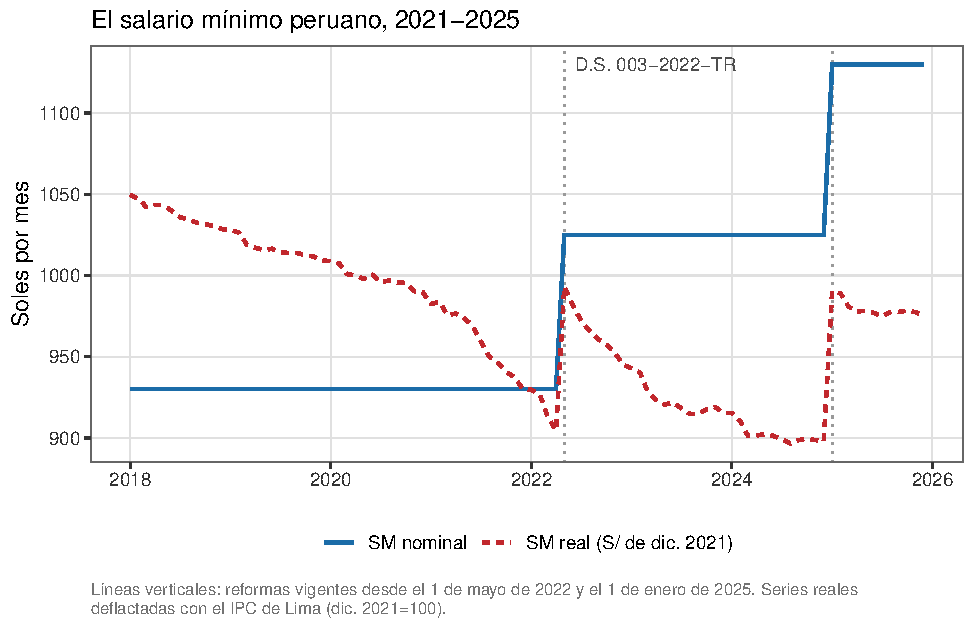
\includegraphics[width=0.82\textwidth]{fig1_minimum_wage.pdf}
\caption{Salario mínimo peruano nominal y real, 2021--2025. La serie real está deflactada por el índice de precios al consumidor de Lima (diciembre de 2021 = 100). Las líneas verticales punteadas marcan las reformas vigentes desde el 1 de mayo de 2022 (Decreto Supremo 003-2022-TR) y el 1 de enero de 2025 (Decreto Supremo 006-2024-TR).}
\label{fig:mw}
\end{figure}

\section{Literatura relacionada}\label{sec:literature}

Este artículo se vincula con tres líneas de investigación: la teoría y la evidencia sobre
los efectos del salario mínimo en el empleo, la evidencia para países en desarrollo con
amplios sectores informales y la literatura específica sobre el Perú.

\paragraph{Teoría y evidencia canónica.} El modelo competitivo predice que un piso salarial
vinculante reduce el empleo de los trabajadores de baja productividad, con un efecto cuyo
tamaño depende de las elasticidades de la demanda de trabajo y de la fracción de
trabajadores alcanzados por el piso \citep{brown_1999}. Los modelos en los que los
empleadores tienen poder para fijar salarios generan predicciones distintas: bajo monopsonio,
un salario mínimo moderado puede elevar el empleo y, por lo general, comprime la cola
inferior de la distribución salarial \citep{manning_2003}. La literatura empírica ha pasado
de presumir efectos de desempleo considerables a un consenso de efectos pequeños en el
margen estudiado. El estudio de caso de \citet{card_krueger_1994} y la síntesis más amplia de
\citet{card_krueger_1995} encontraron poca evidencia de pérdida de empleos por la reforma de
Nueva Jersey, y tanto el diseño de discontinuidad fronteriza de
\citet{dube_lester_reich_2010} como el enfoque de acumulación (\emph{bunching}) de
\citet{cengiz_2019} hallan igualmente que los aumentos recientes en Estados Unidos elevaron
los salarios en la parte baja de la distribución con efectos limitados sobre el empleo;
\citet{manning_2021} interpreta la evidencia acumulada como un efecto sobre el empleo
``esquivo'', mientras que \citet{neumark_wascher_2007} ofrecen la lectura escéptica.
\citet{harasztosi_lindner_2019} muestran que un gran aumento en Hungría se absorbió
principalmente mediante precios y no mediante empleo. Lo más cercano a mi mecanismo es
\citet{dustmann_2022}, quienes muestran que el salario mínimo alemán operó mediante una
\emph{reasignación} que movió trabajadores entre establecimientos, y no mediante pérdidas de
empleo, y \citet{engbom_moser_2022}, quienes documentan cómo el aumento del mínimo brasileño
comprimió la distribución salarial formal; \citet{derenoncourt_montialoux_2021} rastrean las
consecuencias distributivas de las ampliaciones de cobertura en Estados Unidos. Un tema
recurrente, sobre el que construyo directamente, es que los efectos deben medirse allí donde
el mínimo tiene incidencia (\emph{bite}). \citet{card_1992} usa la variación regional en la
fracción de trabajadores afectados, \citet{clemens_wither_2019} siguen a trabajadores cuyos
salarios se encontraban por debajo de un piso federal creciente, \citet{lee_1999} usa la
brecha entre el mínimo y el salario mediano, y \citet{machin_manning_rahman_2003} aprovechan
un sector de bajos salarios en el que la introducción del mínimo en el Reino Unido fue
especialmente vinculante. Mi diseño basado en la educación aplica la misma lógica a una
única reforma nacional.

\paragraph{Países en desarrollo e informalidad.} En economías con amplios sectores
informales, el salario mínimo interactúa con la frontera entre el trabajo cubierto y el no
cubierto, y aparecen repetidamente dos fuerzas opuestas. Un efecto faro puede elevar los
salarios incluso en el sector informal, donde el mínimo funciona como norma o referencia
\citep{lemos_2009, bosch_manacorda_2010, maloney_nunez_2004}, mientras que un efecto de
reasignación puede expulsar a trabajadores del empleo formal hacia arreglos informales o de
trabajo independiente \citep{ham_2018_honduras}; \citet{ulyssea_2018} ofrece el marco de
equilibrio moderno en el que la regulación desplaza a empresas y trabajadores a través de la
frontera de la formalidad. La evidencia latinoamericana abarca todo este rango. Los primeros
trabajos sobre México y Colombia encontraron efectos de desempleo donde el piso era alto en
relación con los salarios \citep{bell_1997}, y \citet{gindling_terrell_2007} muestran para
Costa Rica que los pisos legales mueven los salarios solo en el sector cubierto. Los estudios
sobre Brasil hallan compresión salarial con efectos pequeños sobre el empleo y evidencia de
efectos de derrame hacia el sector informal \citep{lemos_2009, lemos_2004};
\citet{jales_2018} estima, con un enfoque de densidades, que el mínimo brasileño traslada a
una proporción considerable de trabajadores a la informalidad. Los trabajos sobre Ecuador
encuentran efectos salariales positivos concentrados entre los trabajadores de bajos
ingresos \citep{wong_2019_ecuador}, y \citet{arango_2022_colombia} reúnen la evidencia
colombiana reciente. El caso hondureño es el contraejemplo más claro a la visión del efecto
faro: \citet{ham_2018_honduras} documenta que un salario mínimo alto redujo el empleo
cubierto y desplazó a los trabajadores hacia la informalidad, sin reducir la pobreza. Para
Uruguay, \citet{katzkowicz_2021_uruguay} usan un enfoque de discontinuidad en la densidad en
el sector del trabajo doméstico para mostrar que los efectos se concentran entre los menos
calificados. El hilo metodológico común es el uso de medidas de exposición o de incidencia,
ya sean índices de Kaitz geográficos o proporciones de fracción afectada, y una
contabilización cuidadosa del margen informal; adopto ambos elementos.

\paragraph{Perú.} La literatura nacional es escasa y, hasta hace poco, desactualizada; sin
embargo, el margen que enfatizo ha comenzado a recibir atención: \citet{corcuera_2024}
estudia la respuesta del trabajo independiente informal a los aumentos del salario mínimo
peruano con datos anteriores. Los primeros estudios de las reformas de inicios de la década
de 2000 hallan efectos pequeños y a menudo estadísticamente débiles.
\citet{jaramillo_lopez_2006} analizan el aumento de 2003 con paneles trimestrales cortos para
Lima Metropolitana y concluyen que la reforma fue en gran medida inocua, con efectos
negativos sobre la permanencia en el empleo concentrados cerca del piso y evidencia de
desplazamiento del sector formal al informal. \citet{cespedes_2005} estima una elasticidad
del empleo débilmente significativa, de alrededor de $-0.13$, y muestra que la RMV causa en
el sentido de Granger a los salarios formales, una formulación temprana de la visión del
efecto faro para el Perú. El estudio moderno más creíble es \citet{jimenez_2023}, que evalúa
la reforma de 2016 con un diseño de diferencias en diferencias y una dosis de tratamiento a
nivel departamental, definida como la proporción previa a la reforma de trabajadores
formales que ganaban entre el mínimo anterior y el nuevo. Ese estudio no encuentra efectos de
desempleo, halla un aumento de la formalidad de 2.5 a 2.8 puntos porcentuales y ganancias
salariales de 4.1 a 5.4 por ciento, e interpreta este patrón a través del poder de mercado de
los empleadores, del tipo que \citet{amodio_deroux_2021} documentan directamente en plantas
manufactureras colombianas. Mi artículo se diferencia de este precedente en tres aspectos que
hago explícitos. Estudio una reforma posterior y el período posterior a la pandemia; defino
la exposición a nivel de trabajador mediante la educación y no a nivel departamental; y
encuentro un patrón de ajuste distinto, sin ganancia salarial y con una caída, y no un
aumento, de la formalidad. Vuelvo a la conciliación de estos resultados en la
Sección~\ref{sec:discussion}. Como enfatiza \citet{jimenez_2023}, la restricción decisiva para
cualquier diseño peruano es la ausencia de variación subnacional en el mínimo nominal, lo que
obliga al investigador a construir una exposición diferenciada; mi contribución es hacerlo a
través de la dimensión educativa y rastrear sus consecuencias en los márgenes formal e
informal.

\paragraph{Econometría de diferencias en diferencias.} En lo metodológico me apoyo en la
literatura moderna de diferencias en diferencias. Como mi reforma ocurre en una sola fecha,
las preocupaciones recientes sobre ponderaciones negativas y comparaciones prohibidas bajo
adopción escalonada \citep{goodmanbacon_2021, dechaisemartin_2020, sun_abraham_2021,
callaway_santanna_2021} no aplican: con una fecha de tratamiento común, el estimador de
efectos fijos bidireccionales y su análogo de estudio de eventos son insesgados para un
promedio convexo de efectos por grupo y período \citep{roth_2023_trending,
baker_larcker_wang_2022}. Aun así, uso el estimador doblemente robusto de
\citet{santanna_zhao_2020} como pieza de base, y tomo en serio la amenaza a la
identificación, es decir, las tendencias diferenciadas por calificación, mediante el
análisis de sensibilidad de \citet{rambachan_roth_2023}. Para la inferencia con pocos
conglomerados sigo a \citet{bertrand_2004}, \citet{cameron_2008_bootstrap} y
\citet{pustejovsky_tipton_2018}; la selección en la muestra salarial se acota con el enfoque
de recorte de \citet{lee_2009}. Los efectos distributivos se estiman con el método de
cuantiles incondicionales de \citet{firpo_fortin_lemieux_2009}.

\section{Datos y medición}\label{sec:data}

\subsection{Los módulos trimestrales de empleo de la ENAHO}

Utilizo los archivos trimestrales de uso público de la Encuesta Nacional de Hogares (ENAHO), la encuesta nacional de hogares que levanta el Instituto Nacional de Estadística e Informática (INEI) del Perú. La ENAHO es una encuesta representativa a nivel nacional, estratificada y multietápica, con trabajo de campo continuo; el módulo trimestral de empleo e ingresos (módulo 500) registra información detallada del mercado laboral para cada miembro del hogar en edad de trabajar. Agrupo los dieciséis trimestres comprendidos entre el primer trimestre de 2021 y el cuarto trimestre de 2024, alrededor de 347\,000 registros persona-trimestre en total, de los cuales unas 278\,000 observaciones en edad de trabajar y con información de educación ingresan a la muestra de estimación base (se excluye el trimestre de transición 2022Q2, parcialmente tratado; véase la Sección~\ref{sec:strategy}). Para el ejercicio de validación fuera de muestra añado los cuatro trimestres de 2025. Todas las estadísticas usan los factores de expansión del módulo; el tratamiento de los errores estándar se discute en la Sección~\ref{sec:strategy}.

Para el análisis de transiciones a nivel de trabajador de la Sección~\ref{sec:transitions}, complemento los cortes transversales trimestrales con el Panel ENAHO 2020--2024, el componente longitudinal de la encuesta, que vuelve a entrevistar las mismas viviendas cada año e identifica a las mismas personas a lo largo del tiempo. Los pares de años consecutivos enlazan entre 23\,000 y 24\,000 personas, y el INEI publica factores de expansión propios del panel que corrigen por desgaste y no respuesta. El Apéndice~A documenta los archivos fuente, los indicadores de enlace y la construcción de los estados de transición.

La frecuencia trimestral que aprovecho forma parte del diseño de la encuesta y no es una partición ad hoc de un archivo anual. La documentación técnica de la ENAHO establece dos niveles oficiales de inferencia para la muestra integrada: anual (nacional, urbano y rural, cada uno de los 24 departamentos, regiones naturales y Lima Metropolitana) y \emph{trimestral} (nacional, nacional urbano y nacional rural), de modo que el propio diseño muestral respalda la estimación nacional trimestral. Además, en la muestra no panel los mismos conglomerados se visitan en el mismo mes cada año, con viviendas distintas seleccionadas dentro de ellos, por lo que la composición geográfica y estacional de cada trimestre se mantiene fija entre años; en mis archivos, el 70 por ciento de las unidades primarias de muestreo coincide entre el mismo trimestre de años consecutivos, frente a un 5 por ciento entre trimestres distintos. Cada trimestre contiene cerca de la cuarta parte de la muestra anual (alrededor de 1340 conglomerados y entre 21\,000 y 22\,000 registros en edad de trabajar), con una composición estable entre trimestres. La inferencia a nivel departamental, en cambio, solo es anual; por ello, utilizo la variación departamento-trimestre únicamente a través de efectos fijos y celdas agregadas, y mido la incidencia (\emph{bite}) regional agrupando los cinco trimestres previos a la reforma, lo que se aproxima al nivel anual en el que las estimaciones departamentales son representativas.

Restrinjo la muestra a las personas en edad de trabajar, definidas como aquellas de 14 a 65 años,\footnote{Catorce años es la edad mínima legal para trabajar en el Perú; 65 es el límite superior convencional de la población en edad de trabajar.} y elimino las observaciones sin información de educación. El análisis salarial principal se restringe además a los asalariados del sector privado,\footnote{Empleados, obreros y trabajadores del hogar, es decir, la variable de categoría ocupacional de la ENAHO \texttt{p507} igual a 3, 4 o 6; los trabajadores del hogar tienen derecho al salario mínimo desde la Ley 31047 (2020). Los empleadores, los trabajadores por cuenta propia y los trabajadores familiares no remunerados se tratan como categorías aparte, y los trabajadores del sector público se excluyen de los resultados referidos al puesto de trabajo porque su remuneración se rige por escalas propias.} para quienes el salario mínimo es el piso legal relevante, mientras que los resultados de empleo y participación se definen sobre la población en edad de trabajar, y los de formalidad y trabajo independiente, sobre los trabajadores ocupados del sector privado.

\subsection{Educación y definición de los grupos de calificación}

Los grupos de tratamiento y de comparación se definen según el nivel educativo, registrado en la variable \texttt{p301a} de la ENAHO, que recoge el nivel de estudios más alto alcanzado. Validé la codificación de esta variable contra la distribución ponderada del nivel educativo en los datos; corresponde a la clasificación estándar del INEI, que va desde sin nivel hasta posgrado. Defino como trabajadores \emph{poco calificados} a quienes tienen como máximo secundaria completa (sin nivel, inicial, primaria o secundaria), y como \emph{calificados} a quienes tienen algún estudio superior (superior no universitaria, universitaria o posgrado). Excluyo la pequeña categoría residual de educación básica especial, que no se ordena en la dimensión de calificación, y las observaciones sin información de educación.

Esta partición tiene tres rasgos atractivos. Primero, marca una frontera nítida en el mercado laboral peruano: la educación superior es la principal credencial que separa a los trabajadores que compiten por empleos con remuneraciones cercanas al salario mínimo de quienes no lo hacen. Segundo, divide a la población en edad de trabajar en grupos de tamaño comparable, aproximadamente dos tercios de poco calificados y un tercio de calificados, lo que otorga un poder estadístico adecuado a ambos lados. Tercero, y lo más importante para la identificación, los dos grupos difieren marcadamente en su exposición al salario mínimo. Como muestra la Cuadro~\ref{tab:desc}, en el periodo previo a la reforma la mediana del salario mensual de un asalariado poco calificado está cerca del piso legal, mientras que la del asalariado calificado se sitúa muy por encima. La clasificación sigue una larga tradición de trabajos que consideran la educación como un determinante principal de dónde incide el salario mínimo \citep{lemos_2009, katzkowicz_2021_uruguay}.

\subsection{Variables de resultado}

Los resultados se agrupan en tres bloques. En cuanto a la \emph{remuneración}, la ENAHO registra el pago de los asalariados por periodo de pago junto con su frecuencia; dado que más de la mitad de los asalariados de baja educación cobra de forma diaria, semanal o quincenal, frente al quince por ciento de los de alta educación, convierto todos los pagos a equivalentes mensuales con la variable de frecuencia antes de cualquier comparación entre grupos (el Apéndice~\ref{app:data} detalla la conversión, que coincide con la anualización del propio INEI). El salario real por hora divide este ingreso laboral mensual equivalente entre las horas mensuales, se deflacta con el índice de precios al consumidor de Lima del mes al que se refiere el ingreso, en soles de diciembre de 2021, y se winsoriza en el medio percentil inferior y superior; el ingreso mensual real es el mismo numerador sin el ajuste por horas. En cuanto a las \emph{cantidades}, el empleo y la participación laboral son indicadores definidos sobre la población en edad de trabajar, y las horas semanales corresponden a las horas trabajadas en la ocupación principal. En cuanto a la \emph{composición}, el empleo formal y el trabajo independiente se definen entre los trabajadores ocupados del sector privado, y un indicador de percibir menos que el mínimo legal vigente en el mes de referencia del ingreso se define entre los asalariados privados; este último es una medida directa de la incidencia de la política y de su cumplimiento.

La informalidad plantea un problema de medición. El indicador oficial de empleo informal del INEI, \texttt{ocupinf}, figura en los archivos de 2021 a 2023, pero no se publica en los de 2024 y 2025. Como mi ventana de estudio se extiende hasta 2024, reconstruyo un indicador de informalidad consistente a partir de componentes básicos disponibles en todos los años: la afiliación a un sistema de pensiones, la tenencia de un contrato de trabajo formal, la condición de registro de la unidad productiva y la categoría ocupacional. Valido la reconstrucción contra el \texttt{ocupinf} oficial en 2021--2023, años en que ambos están disponibles, y obtengo una coincidencia de alrededor del 88 por ciento a nivel de trabajador, con una tasa de informalidad implícita de 74.9 por ciento frente al 79.1 por ciento oficial. Uso el indicador oficial siempre que existe y la reconstrucción solo para 2024 y 2025, y presento una prueba de robustez que restringe el análisis de formalidad a los años cubiertos por la medida oficial. Los detalles completos de la construcción se encuentran en el Apéndice~\ref{app:data}.

\subsection{Estadísticas descriptivas}

La Cuadro~\ref{tab:desc} presenta las medias ponderadas de las principales variables por grupo de calificación en el periodo previo a la reforma. Los dos grupos difieren en la dirección esperada. Los trabajadores poco calificados son en promedio de mayor edad, con mayor probabilidad están casados y viven en zonas rurales, y tienen salarios mucho más bajos. La tasa de empleo es similar entre grupos, pero la composición del empleo difiere de manera marcada: los poco calificados tienen una probabilidad mucho mayor de ser informales y de trabajar de forma independiente, y una probabilidad mucho mayor de ganar menos que el mínimo legal. Entre los asalariados privados, el 57 por ciento de los poco calificados percibía menos que el \emph{nuevo} mínimo de 1025 soles en la víspera de la reforma, frente al 40 por ciento de los calificados. Esta es la brecha de exposición sobre la que descansa mi diseño, aunque la exposición sustancial del grupo de comparación implica también que el diseño estima un efecto relativo y no absoluto. La alta informalidad del grupo poco calificado, 87 por ciento frente a 53 por ciento entre los calificados, es central para interpretar los resultados: para la mayoría de los trabajadores poco calificados el piso legal no se fiscaliza directamente, de modo que el margen por el que puede ajustarse el mercado laboral es la asignación de los trabajadores entre arreglos formales e informales, y no el nivel de la remuneración dentro de los empleos formales.

\begin{table}[!tbp]\centering
\caption{Estadísticas descriptivas por grupo educativo, período previo a la reforma}\label{tab:desc}
\begin{threeparttable}
\begin{tabular}{lccc}
\toprule
 & Baja educación & Alta educación & Diferencia \\
 & ($\le$ sec. completa) & ($\ge$ superior) & \\
\midrule
Edad & 35.92 & 34.65 & 1.27 \\
Mujer & 0.50 & 0.50 & 0.00 \\
Urbano & 0.76 & 0.93 & -0.17 \\
Casado(a) & 0.53 & 0.41 & 0.12 \\
Años de educación & 8.57 & 14.47 & -5.90 \\
Participación laboral & 0.73 & 0.80 & -0.07 \\
Ocupado & 0.69 & 0.73 & -0.04 \\
Asalariado (incl. del hogar) & 0.29 & 0.48 & -0.19 \\
Independiente & 0.39 & 0.24 & 0.15 \\
Formal (si está ocupado) & 0.13 & 0.47 & -0.34 \\
Informal (si está ocupado) & 0.87 & 0.53 & 0.34 \\
Horas semanales (si está ocupado) & 39.74 & 41.44 & -1.70 \\
Salario real por hora (S/) & 5.74 & 9.08 & -3.34 \\
Ingreso laboral real mensual (S/) & 904.30 & 1\,755.12 & -850.82 \\
Bajo el SM (asalariados) & 0.43 & 0.19 & 0.24 \\
\midrule
Observaciones & 65\,954 & 27\,278 & \\
\bottomrule
\end{tabular}
\begin{tablenotes}\footnotesize
\item Notas: Medias ponderadas con los factores de expansión de la ENAHO; personas en edad de trabajar (14--65) en los trimestres previos a la reforma (2021Q1--2022Q1). Baja educación: a lo sumo secundaria completa (\texttt{p301a}$\le$6). Alta educación: cualquier nivel de educación superior (\texttt{p301a}$\ge$7). Las variables de asalariados (salario por hora, bajo el SM) se condicionan a ser asalariado del sector privado (empleados y trabajadores del hogar, ingresos mensuales equivalentes); las horas y la formalidad se condicionan a estar ocupado. Los conteos de observaciones no están ponderados. La fila de bajo el SM usa el mínimo legal vigente en el mes de referencia del ingreso (930 soles durante toda la ventana previa a la reforma); las proporciones de exposición respecto del NUEVO mínimo (57 frente a 40 por ciento) que se discuten en el texto usan 1025 soles.
\end{tablenotes}
\end{threeparttable}\end{table}


La Figura~\ref{fig:trends} muestra las medias trimestrales ponderadas de los principales resultados por grupo de calificación a lo largo de la ventana de estudio, con la reforma señalada. Las series en bruto ya anticipan los resultados que siguen: las series salariales de ambos grupos se mueven en paralelo durante todo el periodo, mientras que las de formalidad y trabajo independiente empiezan a divergir alrededor de la reforma. La figura deja ver además un hecho que importa para el análisis: en el panel de empleo es la serie de \emph{alta} educación la que oscila, con un fuerte repunte a lo largo de 2021 y vaivenes posteriores, mientras que la serie de baja educación es comparativamente plana, de modo que cualquier ``efecto'' sobre el empleo en el contraste por educación responde en buena medida a los movimientos del grupo de comparación; esta es una de las razones por las que la Sección~\ref{sec:results} no interpreta causalmente ese margen. Se trata de medias no condicionadas; el análisis de regresión que sigue ajusta por composición y estacionalidad.

\begin{figure}[!t]
\centering
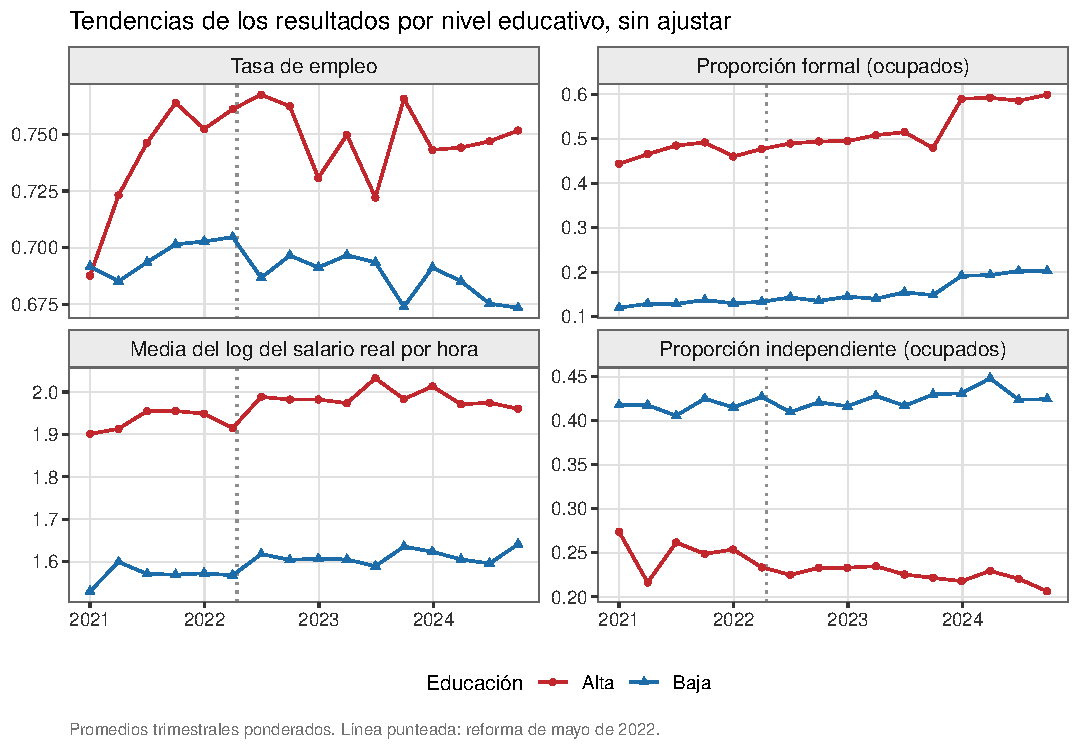
\includegraphics[width=0.95\textwidth]{fig2_raw_trends.pdf}
\caption{Tendencias en bruto de los resultados por grupo de calificación, 2021--2024. Medias trimestrales ponderadas para trabajadores poco calificados y calificados. La línea vertical discontinua señala la reforma de mayo de 2022.}
\label{fig:trends}
\end{figure}

La Figura~\ref{fig:bite} muestra la variación regional en la incidencia del salario mínimo, medida con el índice de Kaitz, el cociente entre el nuevo mínimo y la mediana previa a la reforma del salario mensual equivalente de los asalariados privados en cada departamento. El índice va desde alrededor de 0.79 en Ica hasta cerca de 1.97 en Huánuco, y supera la unidad en dieciocho de los veinticinco departamentos, de modo que en buena parte del país el nuevo mínimo excede la mediana salarial. Esta variación está predeterminada respecto de la reforma y sirve de base para las pruebas de triple diferencia y de intensidad continua de la Sección~\ref{sec:robustness}.

\begin{figure}[!t]
\centering
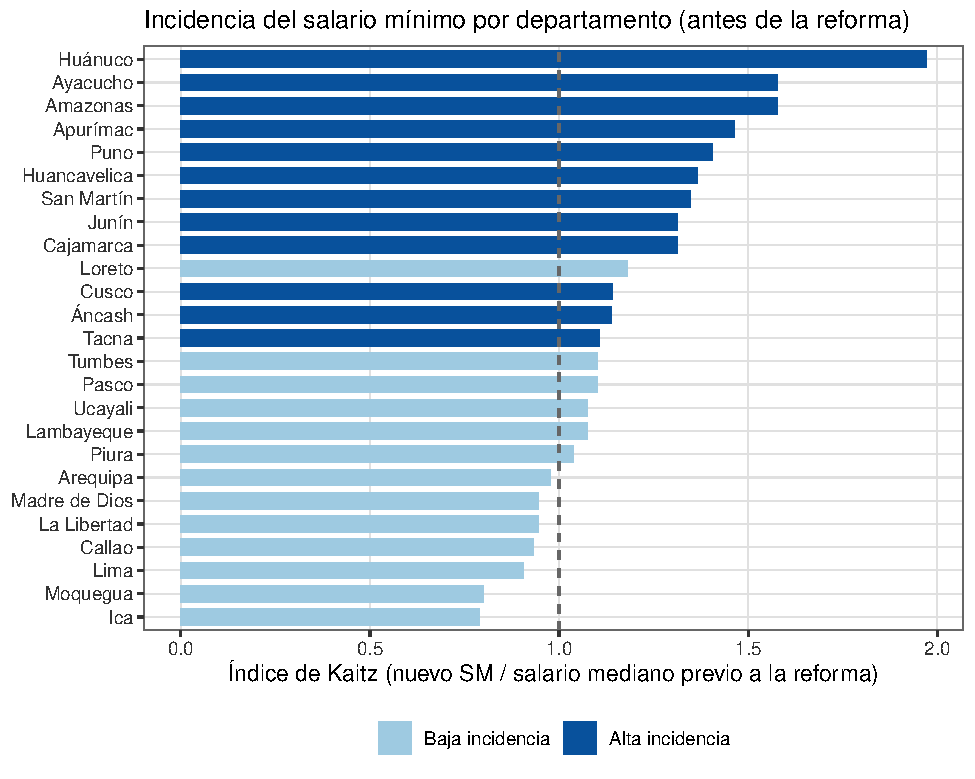
\includegraphics[width=0.72\textwidth]{fig3_regional_bite.pdf}
\caption{Variación regional en la incidencia del salario mínimo. El índice de Kaitz es el cociente entre el nuevo salario mínimo (1025 soles) y la mediana del salario mensual equivalente de los asalariados privados del departamento en los trimestres previos a la reforma. Los departamentos por encima de la línea discontinua tienen una mediana salarial inferior al nuevo mínimo.}
\label{fig:bite}
\end{figure}

\section{Estrategia empírica}\label{sec:strategy}

\subsection{Resultados potenciales y el estimando}

Sea $i$ el índice de individuos, $g\in\{\Low,\mathrm{High}\}$ su grupo de calificación y
$t$ el trimestre. La reforma entra en vigor en el segundo trimestre de 2022, que denoto
$t^{\ast}$;\footnote{Como la reforma rigió desde el 1 de mayo, el segundo trimestre de 2022
contiene un mes previo y dos meses posteriores a la reforma, y los ingresos declarados se
refieren al mes anterior a la entrevista, de modo que incluso las entrevistas de mayo
reportan ingresos previos a la reforma (de abril). Por ello excluyo 2022Q2 de la
especificación base como trimestre de transición parcialmente tratado y lo reincorporo en
una prueba de robustez; el primer trimestre posterior a la reforma en la especificación
base es 2022Q3.} defino el indicador posterior a la reforma
$\Post_t=\mathbf{1}\{t\ge t^{\ast}\}$ y el indicador de tratamiento
$\Low_i=\mathbf{1}\{g_i=\Low\}$. Siguiendo el marco de resultados potenciales, sean
$Y_{it}(1)$ e $Y_{it}(0)$ el resultado del individuo $i$ en el trimestre $t$ con y sin la
reforma vigente. El parámetro de interés es el efecto promedio de la reforma sobre los
trabajadores poco calificados, respecto del contrafactual en el que habrían experimentado
la misma evolución que los calificados,
\begin{equation}
\mathrm{ATT} \;=\; \mathbb{E}\!\left[\,Y_{it}(1)-Y_{it}(0)\;\middle|\;\Low_i=1,\;t\ge t^{\ast}\right].
\end{equation}
Los datos son cortes transversales repetidos y no un panel, de modo que este objeto se
identifica a partir de comparaciones de medias de grupo en el tiempo y no de cambios dentro
de cada persona.

Como el salario mínimo del Perú es nacional y cambia en una sola fecha, no hay variación en
el \emph{momento} del tratamiento: todos los trabajadores quedan expuestos a la misma
política en el mismo instante. La identificación descansa, en cambio, en la variación de la
\emph{intensidad} de la exposición entre grupos de calificación. El diseño es, por tanto, una
diferencias en diferencias canónica de dos grupos con muchos periodos, y no un diseño de
adopción escalonada. Esta distinción importa para la elección del estimador. La literatura
econométrica reciente ha mostrado que el estimador de efectos fijos bidireccionales puede
estar severamente sesgado cuando el momento del tratamiento es escalonado y los efectos son
heterogéneos \citep{goodmanbacon_2021, dechaisemartin_2020, sun_abraham_2021,
callaway_santanna_2021}. Con una fecha de tratamiento común, sin embargo, estos problemas no
se presentan: el estimador de efectos fijos bidireccionales y su análogo de estudio de
eventos recuperan un promedio convexo y correctamente ponderado de los efectos del
tratamiento \citep{roth_2023_trending, baker_larcker_wang_2022}. Aun así, presento el
estimador doblemente robusto de \citet{santanna_zhao_2020} como complemento.

\subsection{Ecuaciones de estimación}

Mi especificación base es el modelo de diferencias en diferencias con efectos fijos
bidireccionales
\begin{equation}
Y_{idt} \;=\; \beta\,(\Low_i\times\Post_t) \;+\; \gamma\,\Low_i \;+\; \lambda_t \;+\; \mu_d
\;+\; X_{it}'\theta \;+\; \varepsilon_{idt},
\label{eq:twfe}
\end{equation}
donde $d$ denota el departamento, $\lambda_t$ son efectos fijos de trimestre, $\mu_d$ son
efectos fijos de departamento y $X_{it}$ es un vector de controles que incluye la edad, su
cuadrado, el sexo, un indicador de zona urbana, el estado civil y los años de educación (que
recogen la variación del nivel educativo dentro de cada grupo de calificación). El
coeficiente $\beta$ es la estimación de diferencias en diferencias. Los efectos fijos de
trimestre absorben cualquier choque común a ambos grupos en un trimestre dado, incluida la
inflación agregada, de modo que las estimaciones en logaritmos no dependen de si los
salarios se expresan en términos nominales o reales deflactados a nivel nacional. Las
observaciones se ponderan con los factores de expansión, y los errores estándar se agrupan
por departamento.

Para trazar la dinámica del efecto y contrastar el supuesto de identificación, estimo la
especificación dinámica de estudio de eventos
\begin{equation}
Y_{idt} \;=\; \sum_{k\neq -1}\beta_k\,\bigl(\Low_i\times\mathbf{1}\{t-t^{\ast}=k\}\bigr)
\;+\; \gamma\,\Low_i \;+\; \lambda_t \;+\; \mu_d \;+\; X_{it}'\theta \;+\; \varepsilon_{idt},
\label{eq:event}
\end{equation}
donde $k$ indexa los trimestres relativos a la reforma y el trimestre inmediatamente anterior
a ella ($k=-1$, el primer trimestre de 2022) es la categoría de referencia omitida. Los
coeficientes $\beta_k$ para $k<0$ miden tendencias previas diferenciales entre los grupos de
calificación y ofrecen una prueba directa de tendencias paralelas; los coeficientes para
$k\ge 0$ trazan la trayectoria del efecto.

\subsection{Supuestos de identificación y amenazas}

La identificación del ATT a partir de la ecuación~\eqref{eq:twfe} requiere que, en ausencia
de la reforma, los resultados de los trabajadores poco calificados y calificados hubieran
seguido trayectorias paralelas, condicionales a los controles y efectos fijos. Tres amenazas
merecen atención.

Primero, las \emph{tendencias diferenciales}. La educación está correlacionada con el sector,
la región y la formalidad, y los dos grupos de calificación podrían haber seguido
trayectorias divergentes por razones ajenas al salario mínimo. Evalúo esto directamente con
los coeficientes del estudio de eventos previos a la reforma y una prueba conjunta de que son
iguales a cero, y examino la robustez a tendencias lineales específicas por departamento.
Como mi ventana se abre en plena recuperación de la pandemia, cuando el empleo de los
trabajadores poco calificados y calificados se recuperó a ritmos distintos, presto especial
atención al primer trimestre de 2021 y presento especificaciones que lo excluyen.

Segundo, la \emph{sensibilidad a violaciones residuales}. Aun cuando las tendencias previas
son estadísticamente planas, no tienen por qué ser exactamente cero. Por ello presento el
análisis de sensibilidad de \citet{rambachan_roth_2023}, que pregunta cuán grande tendría que
ser una violación de tendencias paralelas posterior a la reforma, en relación con la mayor
violación observada antes de ella, para revertir cada conclusión.

Tercero, los \emph{efectos de derrame y de equilibrio general}. Si la reforma desplaza a
trabajadores poco calificados hacia el sector informal, podría deprimir indirectamente los
salarios en ese sector, y si los trabajadores calificados son sustitutos imperfectos, sus
resultados también podrían moverse y contaminar el grupo de comparación. No puedo descartar
esta posibilidad, e interpreto las estimaciones como efectos relativos. El grupo de
comparación no está del todo libre de exposición: el 40 por ciento de los asalariados
privados calificados percibía menos que el nuevo piso antes de la reforma, frente al 57 por
ciento de los poco calificados. En primer orden, esta exposición imperfecta atenúa las
estimaciones hacia cero (el diseño identifica el efecto de la \emph{brecha} de exposición de
diecisiete puntos, por lo que subestima el efecto sobre los plenamente expuestos), pero
reconozco que también convierte las estimaciones en objetos relativos y no absolutos. Por esta
razón complemento el contraste por educación con un diseño de exposición regional continua
que no depende en absoluto del grupo de comparación (Sección~\ref{sec:robustness}).

\subsection{Inferencia}

El tratamiento se asigna a un nivel agregado, el grupo de calificación, lo que plantea la
preocupación habitual de que los errores estándar convencionales sobrestimen la precisión
\citep{bertrand_2004}. La abordo de varias formas complementarias. Mi especificación base
agrupa los errores por departamento,\footnote{Los 25 conglomerados son los 24 departamentos
del Perú más la Provincia Constitucional del Callao. Con pocos conglomerados, los errores
estándar robustos por conglomerado convencionales pueden subestimar la incertidumbre, lo que
motiva las correcciones adicionales que se describen a continuación.} lo que permite una
correlación arbitraria dentro de cada departamento entre individuos y trimestres; presento
una alternativa que agrupa por departamento y grupo de calificación; y aplico la corrección
de muestra pequeña CR2 de reducción de sesgo de \citet{pustejovsky_tipton_2018} a celdas
agregadas a nivel departamental, donde resulta computacionalmente factible. Como estas
correcciones pueden seguir siendo optimistas en un diseño de dos grupos, las complemento con
inferencia por aleatorización a nivel departamental, permutando la incidencia regional del
salario mínimo entre departamentos para construir una distribución nula exacta para el
diseño de intensidad de exposición.

\section{Resultados principales}\label{sec:results}

\subsection{La reasignación del empleo poco calificado}

El resultado central del artículo es que la reforma de 2022 desplazó la composición del
empleo poco calificado desde el trabajo asalariado formal hacia el trabajo independiente,
sin elevar la remuneración de los trabajadores a los que estaba dirigida. Presento primero
la evidencia sobre la composición del empleo, luego la evidencia de primera etapa sobre
dónde el piso es vinculante y, en tercer lugar, la evidencia sobre los salarios.

El efecto estimado sobre la probabilidad de empleo formal entre los ocupados del sector
privado es $-0.046$ (columna 1 del Cuadro~\ref{tab:main}): una caída de 4.6 puntos
porcentuales para los trabajadores poco calificados respecto de los calificados, alrededor
de una quinta parte de la tasa de formalidad de base del grupo, de 23 por ciento. La
semielasticidad implícita es grande (cerca de $-2$ respecto del aumento de 10.2 por
ciento, columna 4 del Cuadro~\ref{tab:main}), pero ello refleja lo reducida que es la base
formal de este grupo y no una respuesta inverosímilmente elástica. La estimación es precisa
con errores agrupados por departamento, y la prueba de tendencias previas no rechaza
tendencias paralelas ($p=0.15$); la Sección~\ref{sec:robustness} toma en serio la
preocupación por una deriva residual y muestra que las magnitudes ajustadas por esa deriva
siguen siendo económicamente grandes y coinciden con la estimación de diferencias en
diferencias sintéticas.
El estudio de eventos de la Figura~\ref{fig:event} muestra que la formalidad relativa de
los poco calificados cae inmediatamente después de la reforma, en alrededor de cuatro
puntos porcentuales en el transcurso de un año, y que la caída persiste. En sentido
inverso, la probabilidad de trabajo independiente aumenta en 3.6 puntos porcentuales. A
diferencia de la formalidad, la serie de trabajo independiente sí rechaza la prueba de
tendencias previas ($p=0.003$), por efecto de un único trimestre elevado a mediados de
2021, por lo que me apoyo en el margen de formalidad como el más limpio de los dos y trato
la estimación de trabajo independiente como su imagen especular, que la corrobora. Las
horas semanales en la ocupación principal aumentan moderadamente y la condición de tiempo
completo disminuye levemente, en línea con un desplazamiento hacia el trabajo por cuenta
propia, donde las horas están menos estandarizadas.

Dos piezas de evidencia independientes respaldan una lectura causal de esta reasignación.
Primero, su magnitud crece con la exposición: como muestra la
Sección~\ref{sec:heterogeneity}, tanto la caída de la formalidad como el aumento del
trabajo independiente son mayores en los departamentos donde el nuevo piso corta más hondo
en la distribución salarial previa a la reforma. Segundo, un diseño de exposición continua
en la línea de \citet{card_1992}, que descarta por completo el contraste por educación y
relaciona los resultados con el índice de Kaitz regional estandarizado previo a la
reforma, arroja el mismo panorama: una incidencia (\emph{bite}) regional una desviación
estándar mayor se asocia con una caída de la formalidad 1.8 puntos porcentuales mayor y con
un aumento del trabajo independiente 1.0 punto mayor después de la reforma, estimaciones
que resisten la inferencia por aleatorización basada en el diseño a nivel de departamento
(Sección~\ref{sec:robustness}). En conjunto, estos resultados describen una reasignación
de los trabajadores poco calificados desde los empleos asalariados formales hacia el
trabajo por cuenta propia, el margen clásico de informalización que destacan
\citet{jaramillo_lopez_2006} para el Perú y \citet{ham_2018_honduras} para Honduras.

\input{../../tables/es/tab_main_did}

\subsection{La primera etapa: donde se fiscaliza, el piso es vinculante}

¿Dónde es realmente vinculante el piso legal? Precisar esto primero ayuda a interpretar
los resultados sobre remuneraciones que siguen. El Cuadro~\ref{tab:firststage} y la
Figura~\ref{fig:bunching} examinan la distribución de ingresos de los asalariados privados
\emph{formales}, el segmento en el que se concentra la fiscalización, en ventanas
simétricas de tres trimestres alrededor de la reforma. Antes de la reforma, 14 por ciento
de los asalariados formales poco calificados percibe un ingreso dentro de un margen de 2.5
por ciento del piso anterior de 930 soles, un pico visible a la manera de
\citet{cengiz_2019} y \citet{engbom_moser_2022}. Después de la reforma, el pico se traslada
prácticamente por completo: la masa en 930 se reduce a menos de 2 por ciento y aparece un
pico casi idéntico, de 14 por ciento, en el nuevo piso de 1025 soles. En otras palabras,
los empleadores del sector formal cumplieron con el nuevo mínimo.

La respuesta de cumplimiento se divide exactamente a lo largo de la frontera de la
fiscalización. El Panel B del Cuadro~\ref{tab:firststage} estima las diferencias en
diferencias para un indicador de remuneración inferior a 1025 soles, manteniendo el umbral
fijo en todos los periodos. Entre los asalariados formales, la proporción por debajo del
nuevo piso cae en cinco puntos porcentuales para los poco calificados respecto de los
calificados (marginalmente significativo, $p=0.10$); entre los asalariados
\emph{informales}, en cambio, \emph{aumenta} en cuatro puntos porcentuales ($p=0.002$): la
remuneración informal se alejó aún más por debajo de un piso que en la práctica no se le
aplica. Ambas respuestas se compensan en la estimación conjunta con umbral fijo (última
fila del Panel B), y por eso tampoco cambia el indicador de remuneración inferior al mínimo
legal del Cuadro~\ref{tab:main}. Junto con los resultados de reasignación, esta evidencia
describe un ajuste coherente entre dos sectores: el piso es vinculante y se respeta dentro
del sector formal, el empleo formal del grupo afectado se contrae y el margen desplazado
reaparece como trabajo independiente y empleo informal, cuya remuneración el piso no
alcanza.

\begin{figure}[!t]
\centering
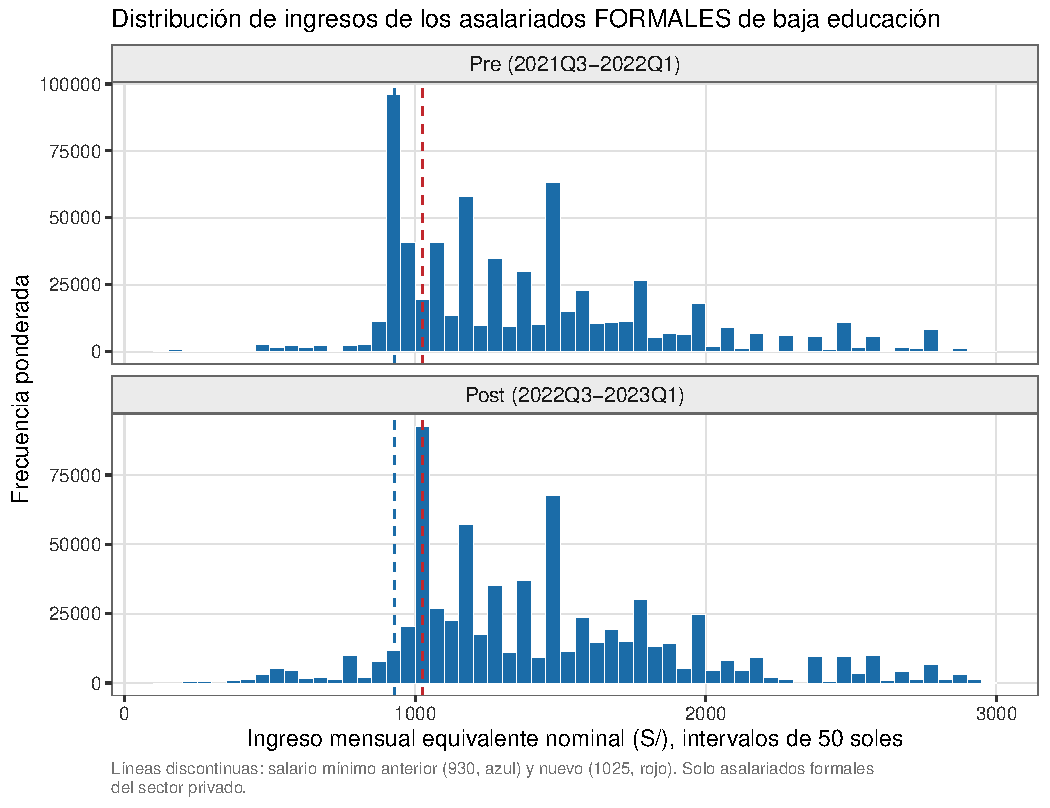
\includegraphics[width=0.8\textwidth]{fig10_bunching.pdf}
\caption{Traslado del pico en el piso salarial entre los asalariados privados formales poco
calificados. Histogramas ponderados de los ingresos nominales equivalentes mensuales
(intervalos de 50 soles) en ventanas simétricas de tres trimestres antes
(2021Q3--2022Q1) y después (2022Q3--2023Q1) de la reforma. Las líneas discontinuas marcan
el salario mínimo anterior (930) y el nuevo (1025).}
\label{fig:bunching}
\end{figure}

\input{../../tables/es/tab_firststage}

\subsection{La respuesta salarial}

Si los empleadores cubiertos cumplieron con el nuevo piso, ¿aumentó la remuneración del
grupo poco calificado en su conjunto? En promedio, no. El coeficiente de la interacción
entre el indicador de baja calificación y el indicador posterior a la reforma es $-0.021$
para el logaritmo del salario real por hora, con un error estándar de $0.012$: negativo,
marginalmente no significativo e incompatible con que la reforma haya elevado la
remuneración relativa. La estimación para el logaritmo de los ingresos mensuales es
igualmente nula. Soy deliberadamente cauto sobre cuánto puede acotar esta regresión, por
una razón transparente que se reporta en la columna (3) del Cuadro~\ref{tab:main}: la
prueba conjunta de tendencias previas para el salario por hora rechaza ($p=0.001$), debido a
un único pico positivo en 2021Q2 ($k=-4$) y no a una tendencia sistemática. Una vez que se
admiten desviaciones de las tendencias paralelas, el contraste por educación no puede
acotar con precisión el efecto salarial en ninguna dirección: bajo la restricción de
magnitudes relativas de \citet{rambachan_roth_2023}, el intervalo robusto con tendencias
paralelas exactas llega a $+2.9$ por ciento, y bajo una extrapolación lineal de la
tendencia previa (levemente decreciente) se admiten valores positivos aún mayores. Por ello
no sustento la conclusión de que la reforma no elevó los salarios en la regresión salarial
promedio. La sustento en las dos piezas de evidencia sobre remuneraciones cuyos
diagnósticos son limpios y que no dependen de la tendencia previa por educación.

Primero, la proporción de asalariados que percibe menos que el piso legal, que era de 35
por ciento entre los asalariados poco calificados en la línea de base, no cae después de la
reforma (la estimación es $-0.006$ con $p=0.45$, y sus tendencias previas son planas,
$p=0.13$). Si las empresas hubieran cumplido con el nuevo piso para el trabajador marginal,
esta proporción habría caído mecánicamente. Segundo, la distribución de ingresos de la
Figura~\ref{fig:dist} muestra una masa visible cerca del mínimo anterior antes de la
reforma, pero ningún traslado apreciable de esa masa hacia el nuevo piso después, lo que
refleja el incumplimiento generalizado documentado en la Sección~\ref{sec:data}; del mismo
modo, las estimaciones por cuantiles incondicionales de la Sección~\ref{sec:heterogeneity}
no muestran ganancias en ningún decil, ni siquiera en los inferiores, donde un piso que se
hace cumplir tendría que comprimir la distribución.

El estimador doblemente robusto de \citet{santanna_zhao_2020} de la columna (2) del
Cuadro~\ref{tab:main} merece una lectura franca y no una nota al pie. Este estimador
colapsa los dieciséis trimestres en una sola comparación antes y después de la reforma y
omite los efectos fijos de departamento, y con errores estándar agrupados por departamento
resulta impreciso para todos los resultados: la estimación salarial es negativa ($-0.056$,
error estándar $0.137$) y la de formalidad es nula ($+0.006$, error estándar $0.040$), en
lugar del $-0.046$ de efectos fijos bidireccionales. Leo esto como el costo conocido de
descartar la estructura temporal \citep{bertrand_2004}: colapsar a dos periodos y
veinticinco conglomerados deja poca variación identificadora, y los intervalos de
confianza resultantes contienen tanto el cero como efectos del doble de mi estimación de
base. Por esta razón trato la columna doblemente robusta como una verificación
complementaria conservadora y no como la estimación preferida, y la corroboración en la
que me apoyo proviene, en cambio, de diseños que conservan variación independiente: la
estimación de diferencias en diferencias sintéticas sobre celdas departamentales y el
diseño de exposición regional continua de la Sección~\ref{sec:robustness}.

Que la reforma no haya elevado los salarios en la parte baja de la distribución no
sorprende en este contexto: descontada la inflación, el valor real del piso aumentó poco, la
mayoría de los trabajadores poco calificados es informal o trabaja de manera independiente,
y la fiscalización es escasa, de modo que el mínimo legal restringe la remuneración solo de
una minoría. La ausencia de respuesta en las remuneraciones contrasta con el patrón de
``efecto faro'' que \citet{jimenez_2023} encuentra para la reforma de 2016. Retomo estos
mecanismos, y el contraste con reformas anteriores, en la Sección~\ref{sec:discussion}.


\subsection{El nivel de empleo}

El efecto estimado sobre la tasa de empleo total es de $-2.5$ puntos porcentuales, lo que
implicaría una elasticidad del empleo respecto del salario mínimo de alrededor de $-0.35$,
más del doble de las estimaciones más altas de la literatura peruana previa
\citep{cespedes_2005}. No doy a esta estimación una interpretación causal, por tres razones
documentadas en la Sección~\ref{sec:robustness}: la serie de empleo presenta una clara
tendencia previa diferencial, asociada a la recuperación tras la pandemia y concentrada a
inicios de 2021 ($p<0.001$ en la prueba de tendencias previas); reformas placebo ubicadas
en el periodo previo producen ``efectos'' de magnitud y significancia similares; y, a
diferencia de los márgenes de composición, el efecto sobre el empleo no crece con la
exposición regional; en todo caso, es menor en los departamentos de alta incidencia. Al
excluir 2021Q1, la estimación puntual se reduce aproximadamente a la mitad y no sobrevive a
los procedimientos de inferencia más conservadores. Por lo tanto, interpreto el resultado
sobre el nivel de empleo como reflejo de dinámicas de recuperación diferenciales y no del
salario mínimo, y concentro el peso interpretativo en el desplazamiento de la composición,
cuyos diagnósticos son limpios.

\subsection{Transiciones individuales: el margen de entrada}\label{sec:transitions}

Los resultados de composición describen stocks netos. Para identificar el flujo bruto que
los origina, complemento los cortes transversales repetidos con la ENAHO Panel 2020--2024,
que vuelve a entrevistar anualmente a las mismas viviendas y enlaza a las personas entre
años (Sección~\ref{sec:data}; los detalles de construcción están en el Apéndice~A). Apilo
los cuatro pares de años consecutivos, de 2020--21 a 2023--24, y clasifico cada par respecto
de la reforma según el mes de entrevista de 2022: pares previos a la reforma; pares de la
ventana de reforma, cuyo estado de origen se mide antes de mayo de 2022 y cuyo destino se
mide después; y pares posteriores a la reforma. Entre los trabajadores con un empleo
privado formal en el año base, estimo unas diferencias en diferencias apiladas para cada
estado de destino, con efectos fijos de par y de departamento, controles individuales,
ponderadores del panel que corrigen la atrición y errores estándar agrupados por
departamento. El Cuadro~\ref{tab:transitions} reporta las proporciones de destino y las
estimaciones.

Dos hallazgos precisan el mecanismo. Primero, los trabajadores en su puesto no fueron
expulsados. Respecto de los trabajadores formales de alta educación, la probabilidad de
que un trabajador formal de baja educación siga siendo formal \emph{aumenta} a lo largo de
la ventana de reforma (8.3 puntos porcentuales, $p=0.055$), y la transición hacia el empleo
asalariado informal cae ($-4.8$ puntos, $p=0.076$); las transiciones hacia el trabajo
independiente y hacia el no empleo no se mueven. Esto es exactamente lo que implica la
primera etapa: dentro del segmento fiscalizado, los trabajadores en su puesto recibieron el
aumento obligatorio y conservaron su empleo. Segundo, la puerta de entrada se cerró. Entre
quienes tenían un empleo informal en el año base, la probabilidad de que un trabajador de
baja educación pase \emph{a} un empleo privado formal cae en 2.1 puntos porcentuales
($p=0.011$) en los pares posteriores a la reforma, casi la mitad de la tasa de entrada de
base del grupo, de 4.5 por ciento. La caída del stock de formalidad documentada en la
Sección~\ref{sec:results} es, por lo tanto, un fenómeno del margen de las contrataciones:
la reforma no disolvió los vínculos formales existentes, sino que redujo el ritmo al que se
creaban otros nuevos para los trabajadores de baja educación. Esta lectura es coherente con
la incidencia de los efectos de composición entre los jóvenes, las mujeres y los perceptores
secundarios de ingreso, los trabajadores con mayor probabilidad de ser entrantes marginales
y no trabajadores protegidos en su puesto.

Tres salvedades acotan esta evidencia. El panel es anual, por lo que no puedo fechar las
transiciones dentro del año más allá de la división por mes de entrevista; los pares de
referencia previos a la reforma incluyen transiciones desde el año de la pandemia, 2020,
que tuvieron una rotación inusual; y la muestra con base formal es modesta (unas 7000
observaciones de pares), de modo que la estimación de permanencia es solo marginalmente
significativa. La respuesta de entrada aparece en los pares posteriores a la reforma y no
en la ventana inmediata de la reforma, lo que es coherente con flujos de contratación que se
ajustan con rezago. Por ello leo la evidencia del panel como una corroboración cualitativa
del mecanismo (permanencia de los trabajadores en su puesto más una menor entrada a la
formalidad) y no como magnitudes precisas.

\input{../../tables/es/tab_transitions}

\begin{figure}[!t]
\centering
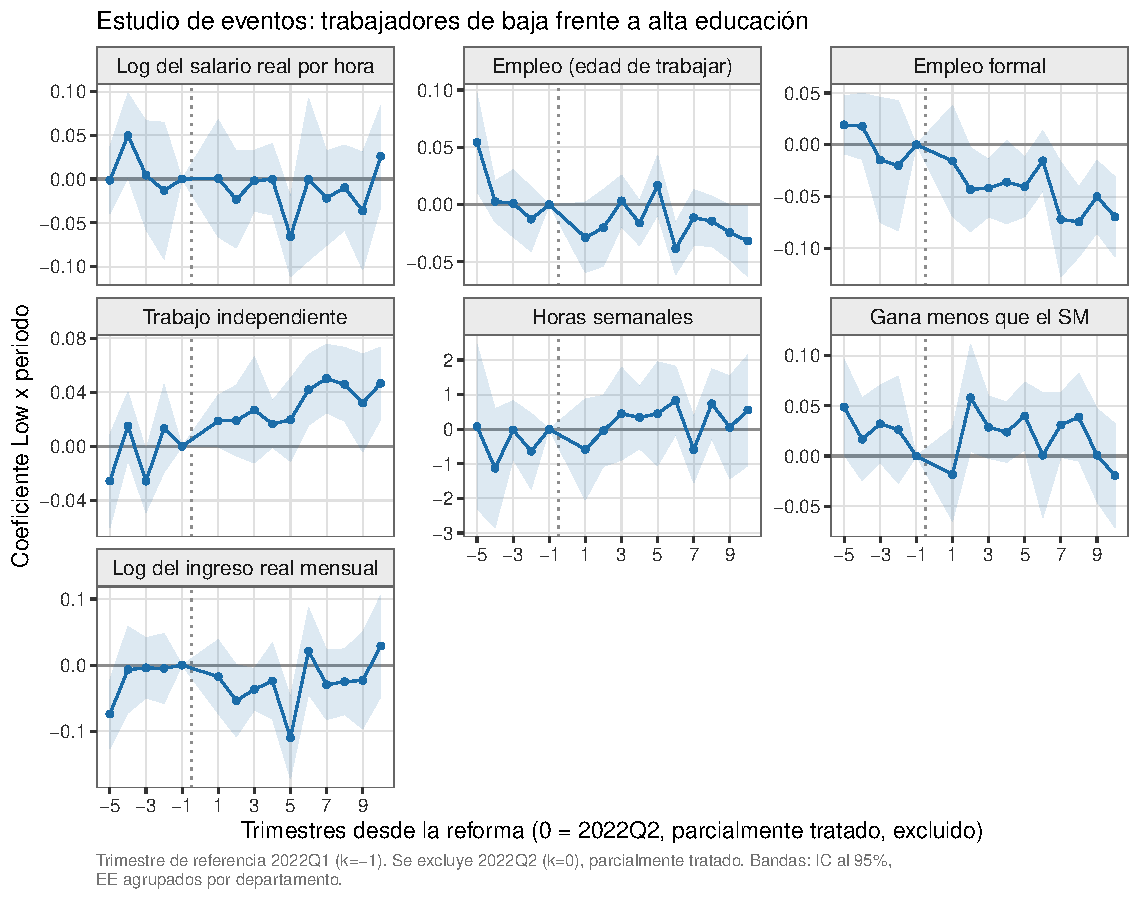
\includegraphics[width=0.98\textwidth]{fig5_event_study.pdf}
\caption{Estimaciones del estudio de eventos de la reforma de 2022. Cada panel grafica los
coeficientes $\beta_k$ de la interacción entre el indicador de baja calificación y los
indicadores trimestrales de la ecuación~\eqref{eq:event}, respecto del trimestre omitido
2022Q1 ($k=-1$). Se excluye el trimestre de transición 2022Q2 ($k=0$), parcialmente
tratado. Las bandas sombreadas son intervalos de confianza al noventa y cinco por ciento con
errores estándar agrupados por departamento.}
\label{fig:event}
\end{figure}

\begin{figure}[!t]
\centering
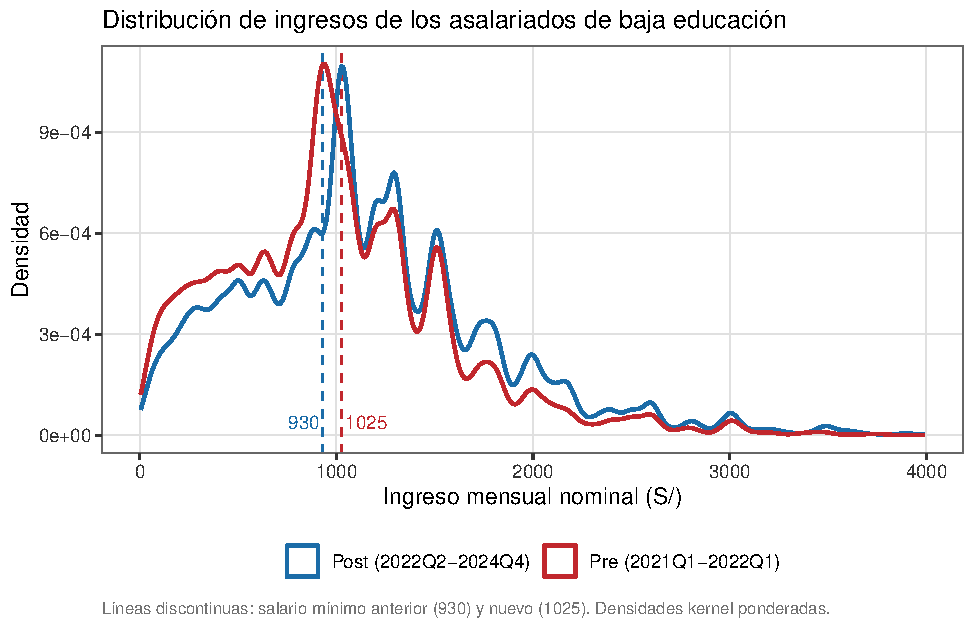
\includegraphics[width=0.72\textwidth]{fig4_wage_distribution.pdf}
\caption{Distribución de ingresos de los asalariados poco calificados, antes y después de
la reforma. Densidades kernel ponderadas de los ingresos nominales equivalentes mensuales
(empleados del sector privado y trabajadores del hogar), con el salario mínimo anterior
(930) y el nuevo (1025) marcados con líneas discontinuas.}
\label{fig:dist}
\end{figure}

\section{Robustez e inferencia}\label{sec:robustness}

En esta sección someto los resultados principales a una batería de pruebas de
especificación, de inferencia y de diseño, y luego a una replicación fuera de muestra. El
mensaje general es que los resultados de composición, la caída de la formalidad y el
aumento del trabajo independiente, son los hallazgos más robustos, y los corrobora un
diseño independiente de exposición continua con inferencia por aleatorización; la
evidencia salarial muestra de forma consistente que no hubo ganancias de remuneración,
aunque con una salvedad sobre las tendencias previas; y el resultado sobre el nivel de
empleo no supera sus diagnósticos y no debe leerse como causal.

\subsection{Robustez a la especificación}

El Cuadro~\ref{tab:robspec} reporta el coeficiente $\mathrm{Low}\times\mathrm{Post}$ para
los cuatro resultados principales bajo diez especificaciones alternativas: sin controles;
sin el trimestre pandémico de inicios de 2021; con tendencias lineales específicas por
departamento; restringiendo la muestra a trabajadores en edad central; con un corte
educativo alternativo que elimina las categorías situadas en la frontera entre ambos
grupos; con efectos fijos de ocupación y de rama de actividad; agrupando los errores por
departamento y nivel de calificación; reincorporando el trimestre de transición 2022Q2,
parcialmente tratado; excluyendo la agricultura (cubierta por el régimen laboral agrario
de la Ley 31110 y no por el salario mínimo general); y reincorporando a los trabajadores
del sector público en las muestras condicionadas a tener empleo. Las estimaciones de
formalidad y de trabajo independiente son estables en signo y magnitud en todos los
casos y se mueven dentro de un rango estrecho. La estimación salarial es negativa o nula
en todas las especificaciones y nunca es significativamente positiva. La estimación de
empleo, en cambio, se atenúa notablemente cuando se excluye el trimestre pandémico o se
incluyen tendencias específicas por departamento, lo que refuerza mi renuencia a
interpretarla de manera causal.

\input{../../tables/es/tab_robustness}

\subsection{Inferencia}

Como el contraste de tratamiento varía solo entre dos grupos educativos, el
agrupamiento convencional por departamento no proporciona por sí solo una inferencia
basada en el diseño para el coeficiente $\mathrm{Low}\times\mathrm{Post}$; por ello
reporto un conjunto de procedimientos cada vez más exigentes. El
Cuadro~\ref{tab:inference} reúne la evidencia. Las columnas (1) a (3) reportan los
valores $p$ del efecto base con errores agrupados por departamento (25 conglomerados),
por departamento y nivel de calificación (50 conglomerados), y con la corrección CR2
para muestras pequeñas de \citet{pustejovsky_tipton_2018}, aplicada a celdas colapsadas
en el espíritu de \citet{bertrand_2004}, aquí al nivel
departamento$\times$grupo$\times$periodo, que es la agregación más fina en la que la
corrección CR2 resulta computacionalmente factible.
Los efectos sobre la formalidad y el trabajo independiente siguen siendo altamente
significativos bajo ambos esquemas de agrupamiento; con el procedimiento CR2 sobre
celdas colapsadas, deliberadamente conservador y de baja potencia con veinticinco
departamentos, el trabajo independiente sigue siendo marginalmente significativo y la
formalidad no. El efecto sobre el empleo pierde significancia con cualquier
procedimiento más exigente que el simple agrupamiento por departamento. Como una prueba
de permutación del contraste entre dos grupos no está definida, la inferencia por
aleatorización basada en el diseño se aplica, en su lugar, al diseño de exposición
continua, donde la asignación que se permuta (la incidencia regional) toma veinticinco
valores: la columna (4) reporta estos valores $p$, que corresponden a las estimaciones
de la columna (5) y no al contraste educativo.\footnote{Un \emph{wild cluster
bootstrap} en el espíritu de \citet{cameron_2008_bootstrap} no está disponible para
estimaciones ponderadas con factores de expansión, de modo que los procedimientos CR2 y
de aleatorización cumplen aquí ese papel.}

\input{../../tables/es/tab_inference}

\subsection{Robustez del diseño: intensidad de la incidencia y triples diferencias}

Mi identificación descansa en la exposición diferencial por nivel educativo, pero el
salario mínimo también tiene una incidencia (\emph{bite}) distinta entre regiones, y esto
ofrece una fuente independiente de variación que no depende en absoluto del contraste
educativo. La columna (5) del Cuadro~\ref{tab:inference} reporta una especificación de
exposición continua en el espíritu de \citet{card_1992}, que relaciona los resultados
con el índice de Kaitz departamental previo a la reforma, estandarizado e interactuado
con el indicador del periodo posterior. Los resultados corroboran el diseño basado en la
calificación en los márgenes de composición: en los departamentos donde el salario
mínimo incide con más fuerza, tras la reforma el empleo formal cae 1.8 puntos
porcentuales más por cada desviación estándar de exposición ($p<0.001$; $p$ por
aleatorización $<0.001$) y el trabajo independiente aumenta 1.0 punto más ($p=0.02$;
$p$ por aleatorización $=0.02$). En este diseño el empleo también disminuye con la
exposición, aunque descarto ese margen por las razones ya expuestas. Los salarios no
muestran una respuesta significativa. Una especificación de triple diferencia que
interactúa el contraste por calificación con un indicador de departamentos de alta
incidencia no es estadísticamente significativa para ningún resultado (Cuadro del
Apéndice~\ref{tab:ddd}); lo interpreto como falta de potencia de una partición regional
binaria y gruesa, más que como evidencia contra el mecanismo, dado que la versión
continua es informativa y que las estimaciones por subgrupos de la
Sección~\ref{sec:heterogeneity} se mueven en la dirección esperada.

Otras tres pruebas de diseño matizan esta corroboración (Cuadros del
Apéndice~\ref{tab:expocells} y~\ref{tab:sectorocc}). En primer lugar, el diseño regional
supera su propio diagnóstico de adelantos justo donde importa: las pruebas conjuntas de
las interacciones trimestre$\times$exposición previas a la reforma no rechazan la nula
para la formalidad ($p=0.84$), el trabajo independiente ($p=0.20$) ni los salarios
($p=0.24$), y solo la rechazan para el empleo ($p=0.002$), lo que es coherente con todo
lo demás que sabemos de ese margen. En segundo lugar, en aras de la plena
transparencia, estimo también diseños más finos de fracción afectada a nivel de celda
\citep{card_1992, clemens_wither_2019}, con la exposición medida dentro de celdas
departamento$\times$calificación$\times$edad; ambas variantes fallan sus diagnósticos de
adelantos: la exposición de grano fino se confunde con las heterogéneas recuperaciones
pospandemia de las celdas, y la variante entre pisos incluso invierte los signos, porque
las celdas con masa entre ambos pisos son precisamente las celdas semiformales que se
recuperaron más rápido. Por ello, trato al departamento como el nivel creíble para la
variación de la exposición y reporto los diseños por celda en el apéndice en lugar de
omitirlos. En tercer lugar, la reasignación es amplia entre sectores: la caída de la
formalidad aparece por igual en los sectores cubiertos de alta incidencia, en los demás
sectores privados y en la agricultura. La estimación agrícola no es una falla de
falsificación, porque la remuneración diaria del régimen agrario está indexada a la RMV
y, por tanto, subió con la reforma; en el Perú ningún sector grande queda con su piso
sin cambios, y por eso los contrastes de cobertura no pueden ser nítidos en este caso.
Una relación dosis-respuesta a nivel de ocupación (con la exposición medida como la
proporción de asalariados de la ocupación que ganaban menos que el nuevo piso antes de
la reforma) muestra mayores caídas en la remuneración por debajo del piso y, de manera
sugerente, ganancias salariales relativas en las ocupaciones más expuestas, aunque la
ocupación se mide después del tratamiento y leo ese panel como descriptivo.

Como prueba final de diseño, estimo diferencias en diferencias sintéticas
\citep{arkhangelsky_2021_sdid} sobre celdas departamento-trimestre, tratando a los
departamentos de alta incidencia como tratados desde 2022Q3 y dejando que el estimador
repondere a los departamentos de baja incidencia para reconstruir su trayectoria previa
a la reforma (Cuadro del Apéndice~\ref{tab:sdidpower}). Las estimaciones van en la
dirección de la reasignación (la formalidad cae y el trabajo independiente sube, ya sea
que el resultado sea la media de baja educación o la brecha entre baja y alta
calificación), con magnitudes de aproximadamente la mitad de las estimaciones TWFE y una
precisión limitada por las veinticinco unidades agregadas; la caída de la formalidad en
las medias de baja educación es significativa al cinco por ciento con el
\emph{jackknife}.

\subsection{Selección y potencia}

Como la reforma sacó a trabajadores de la muestra de asalariados, las diferencias en
diferencias salariales se condicionan a una población endógena. El Cuadro del
Apéndice~\ref{tab:leemde} acota el sesgo resultante con el método de recorte de
\citet{lee_2009}: la reforma redujo la inclusión de los trabajadores poco calificados en
la muestra salarial en 2.1 puntos porcentuales (7.6 por ciento de la tasa base), y
recortar en esa fracción la distribución salarial low$\times$post desde cualquiera de
sus colas acota las diferencias en diferencias salariales 2$\times$2 no condicionadas
entre $-0.10$ y $+0.10$. La selección por sí sola podría, entonces, ocultar efectos
salariales de hasta diez puntos logarítmicos en cualquier dirección, lo cual es una
declaración franca de lo que la evidencia salarial puede y no puede descartar; la
evidencia de cumplimiento y de acumulación (\emph{bunching}) de la
Sección~\ref{sec:results}, que solo condiciona en la condición de formalidad, no está
sujeta a esta preocupación, y es en ella donde apoyo la conclusión sobre la
fiscalización. El mismo cuadro del apéndice reporta los efectos mínimos detectables: con
una potencia del ochenta por ciento, el diseño puede detectar efectos salariales de 3.4
puntos logarítmicos y efectos de 2.1 y 1.7 puntos porcentuales sobre la formalidad y el
trabajo independiente, ambos muy por debajo de los estimados de 4.6 y 3.6, de modo que
los hallazgos de composición no son un artefacto de una baja potencia estadística.

La misma lógica de selección se aplica a los propios resultados de composición, que se
definen entre los ocupados, mientras que el margen de empleo arrastra una tendencia
previa ligada a la recuperación. Por ello, el Cuadro del Apéndice~\ref{tab:uncond}
reporta versiones no condicionadas, definidas como proporciones de la población en edad
de trabajar, que no condicionan en el empleo. En el contraste educativo, las
estimaciones no condicionadas son mayores (empleo formal $-3.3$ puntos, trabajo
independiente $+1.7$), pero heredan la tendencia previa diferencial de recuperación
pospandemia del margen de empleo y no superan su diagnóstico, de modo que las reporto
por transparencia, sin apoyarme en ellas. El resultado informativo está en el diseño
regional, que no usa el contraste educativo: el empleo formal no condicionado cae 1.6
puntos porcentuales por cada desviación estándar de exposición ($p$ por aleatorización
$<0.001$), de modo que la caída del empleo formal no es un artefacto de condicionar en
una población ocupada cambiante. El trabajo independiente no condicionado, en cambio, no
aumenta con la exposición regional; en ese diseño, el aumento de la \emph{proporción}
del trabajo independiente en el empleo opera a través de la reducción del denominador de
empleo, y la reasignación absoluta hacia el trabajo independiente es un rasgo propio del
contraste educativo. Retomo esta distinción en la Sección~\ref{sec:discussion}.

\subsection{Sensibilidad a violaciones de las tendencias paralelas}

Incluso unas tendencias previas planas se estiman con error, por lo que aplico el
análisis de sensibilidad de \citet{rambachan_roth_2023}. La Figura~\ref{fig:honest}
muestra el conjunto de confianza robusto para el efecto promedio posterior a la reforma
sobre el empleo y la formalidad, cuando permito que la violación posterior de las
tendencias paralelas sea tan grande como un múltiplo $\bar{M}$ de la mayor violación
previa a la reforma. Los efectos sobre la formalidad y el trabajo independiente se
mantienen alejados de cero bajo tendencias paralelas exactas, pero incluyen el cero en
cuanto se admiten violaciones de apenas $\bar{M}=0.1$, y el efecto sobre el empleo
incluye el cero incluso con $\bar{M}=0$. Este es el eslabón más débil del diseño
basado en la educación, y lo digo con claridad: los resultados de composición son
robustos a la inferencia convencional y a la basada en el diseño, pero no a violaciones
moderadas de las tendencias paralelas en el contraste educativo. Su credibilidad
descansa, por lo tanto, en las dos piezas de evidencia que no dependen de ese contraste:
el gradiente regional de dosis-respuesta y el diseño de exposición continua con
inferencia por aleatorización. El cálculo de potencia de \citet{roth_2022_pretest}
cuantifica por qué no me apoyo solo en haber superado las pruebas previas: una violación
lineal de las tendencias paralelas que mi prueba previa detectaría solo la mitad de las
veces sesgaría el efecto promedio sobre la formalidad en el periodo posterior en 0.042,
nueve décimas del efecto estimado (Cuadro del Apéndice~\ref{tab:sdidpower}, Panel B).
Superar las pruebas previas da tranquilidad, pero no es concluyente, y así las trato a
lo largo de todo el artículo.

La granularidad temporal tampoco determina las estimaciones. Los estudios de eventos
mensuales (Figura~\ref{fig:monthly}), que fechan los resultados salariales según el mes
de referencia del ingreso y los de empleo según el mes de la entrevista, muestran que la
caída de la formalidad aparece inmediatamente después de mayo de 2022 y persiste, con
una caída sugerente en las semanas en torno a la publicación del decreto, el 3 de abril;
y un estudio de eventos trimestral que agrupa la cola derecha en $k\ge 8$, en lugar de
estimar once rezagos libres, deja las estimaciones sin cambios.\footnote{Las series
completas de coeficientes mensuales y agrupados se incluyen en el paquete de
replicación.}

\begin{figure}[!t]
\centering
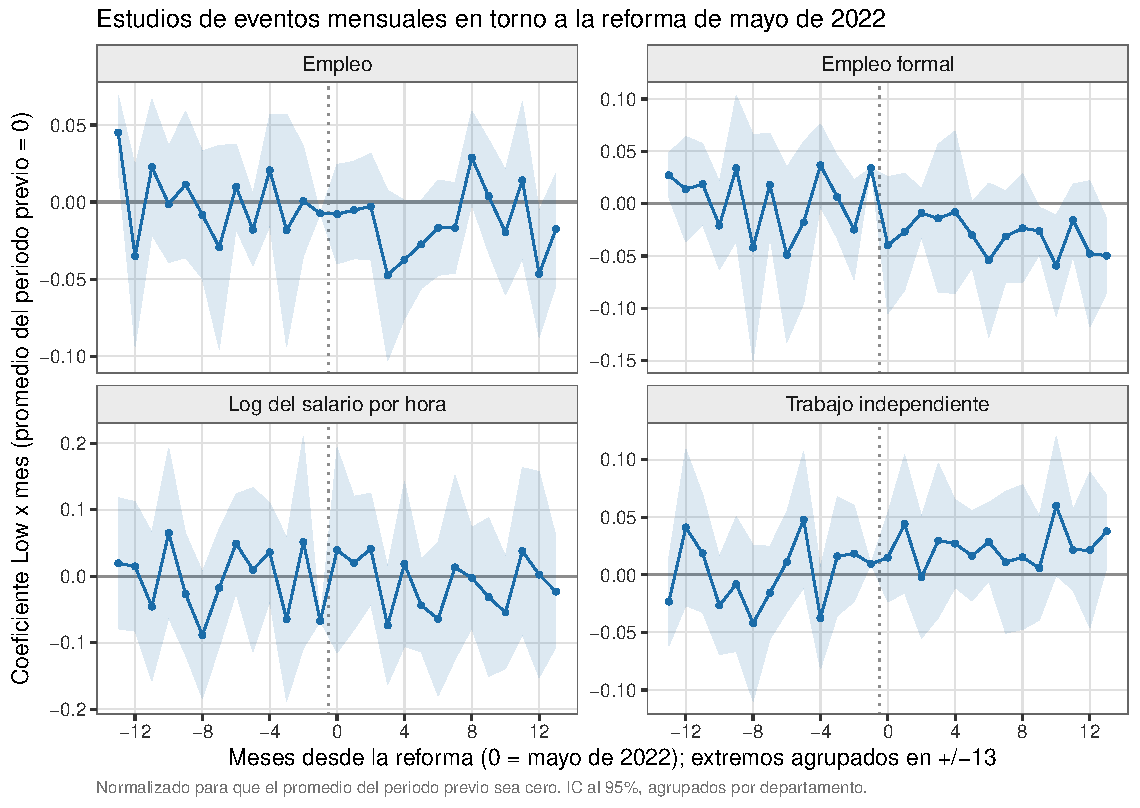
\includegraphics[width=0.98\textwidth]{fig11_monthly_event.pdf}
\caption{Estudios de eventos mensuales en torno a la reforma de mayo de 2022. Los
resultados salariales se fechan según el mes de referencia del ingreso y los de empleo
según el mes de la entrevista; extremos agrupados en $\pm$13 meses; mes de referencia:
abril de 2022. Bandas: intervalos de confianza al 95 por ciento con errores agrupados
por departamento.}
\label{fig:monthly}
\end{figure}

\begin{figure}[!t]
\centering
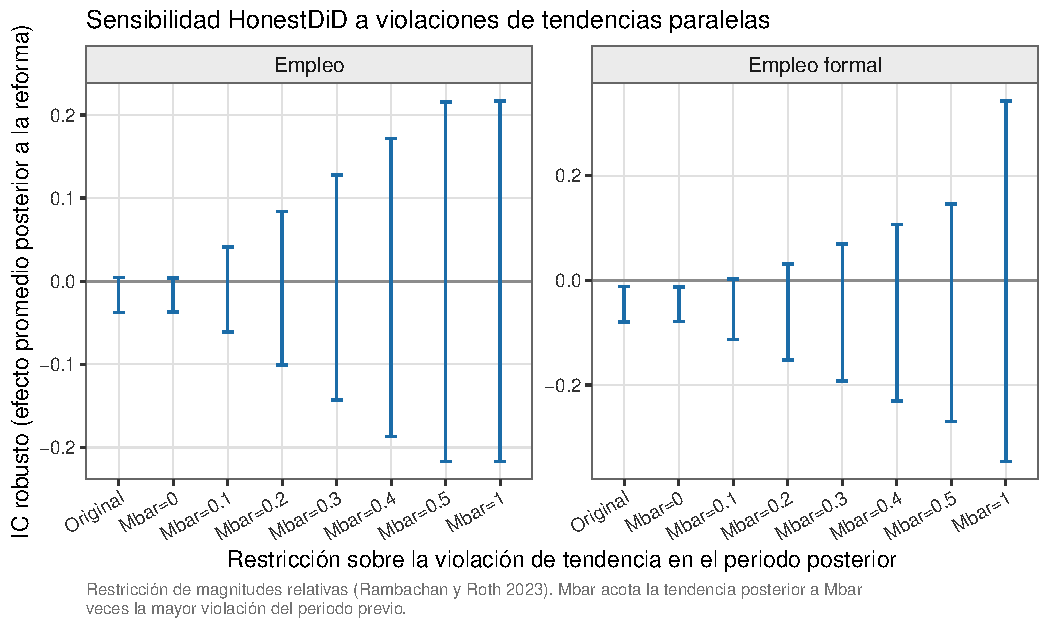
\includegraphics[width=0.8\textwidth]{fig7_honestdid.pdf}
\caption{Sensibilidad a violaciones de las tendencias paralelas
\citep{rambachan_roth_2023}. Conjuntos de confianza robustos para el efecto promedio
posterior a la reforma bajo la restricción de magnitudes relativas, que acota la
violación de la tendencia posterior a la reforma en $\bar{M}$ veces la mayor violación
previa a la reforma.}
\label{fig:honest}
\end{figure}

\subsection{Reformas placebo y exclusión de una unidad a la vez}

Asigno reformas ficticias a cada trimestre interior de la ventana previa a la reforma y
vuelvo a estimar las diferencias en diferencias usando solo datos previos a la reforma
(Cuadro del Apéndice~\ref{tab:placebo}). Los placebos salariales son nulos y los del
trabajo independiente son marginales en dos de los tres trimestres. Los placebos de
empleo son grandes y significativos en los tres trimestres, lo cual es un síntoma
directo de la tendencia previa impulsada por la pandemia en ese resultado y la base de
mi negativa a interpretar causalmente la estimación de empleo.

Los placebos de formalidad merecen algo más que una lectura de aprobado o desaprobado,
porque ellos y la prueba conjunta de tendencias previas responden la misma pregunta con
distinta potencia. Los tres son negativos ($-0.024$, $-0.029$, $-0.017$, el último
significativo al cinco por ciento): aunque la prueba conjunta no rechaza la nula
($p=0.15$), el patrón de las estimaciones puntuales indica una deriva relativa a la baja
de aproximadamente dos puntos porcentuales a lo largo de la ventana previa. Por eso
cuantifico cómo cambia la estimación de formalidad bajo correcciones de la deriva de
severidad creciente, en lugar de apoyarme solo en haber superado la prueba. Descontar
aritméticamente la deriva implícita en los placebos deja un efecto de aproximadamente
$-0.02$ a $-0.03$, que sigue siendo más de una décima parte de la formalidad base y que
está muy cerca de la estimación de la brecha por calificación con diferencias en
diferencias sintéticas ($-0.028$), inmune por construcción a una deriva a nivel de
grupo. Dos correcciones más agresivas acotan los extremos. Una especificación que
permite que los dos grupos educativos diverjan según una tendencia lineal libre a lo
largo de toda la ventana (Cuadro~\ref{tab:robspec}) lleva a cero las estimaciones de
composición del contraste educativo, pero esto es mecánico y no diagnóstico: un cambio
de nivel inmediato y persistente, observado durante diez trimestres posteriores a la
reforma, se aproxima bien mediante una tendencia, de modo que esta especificación
absorbe un verdadero efecto escalón junto con cualquier deriva y conviene leerla como
el peor escenario. De manera simétrica, la restricción de suavidad de
\citet{rambachan_roth_2023}, que extrapola la tendencia previa lineal ajustada al
periodo posterior, produce un intervalo no informativo para la formalidad
($[-0.045,\,0.041]$ con $M=0$): extrapolar cuatro puntos ruidosos del periodo previo a
lo largo de diez trimestres posteriores dispara la varianza. El resumen justo es que el
contraste educativo, por sí solo, no puede separar un cambio de nivel persistente de una
tendencia de grupo en una ventana tan larga. Precisamente por eso el peso causal de este
artículo descansa en el diseño de exposición regional, cuyos adelantos son planos, cuya
inferencia se basa en el diseño y cuyo gradiente de dosis-respuesta no puede ser
generado por una deriva específica de grupo; y en la convergencia de la estimación
educativa ajustada por la deriva con la estimación de diferencias en diferencias
sintéticas, de $-0.02$ a $-0.03$.

La reestimación excluyendo un departamento a la vez y excluyendo un trimestre a la vez
(Cuadro del Apéndice~\ref{tab:loo}) deja las estimaciones puntuales prácticamente sin
cambios para los cuatro resultados, lo que indica que ninguna región ni ningún
trimestre en particular determina los resultados.

\subsection{La ola de inmigración venezolana}

Un choque distinto de oferta laboral se superpone a mi contexto: el éxodo venezolano
trajo al Perú alrededor de 1.5 millones de migrantes, concentrados en 2018--2019 y en
Lima y la costa urbana, que compiten sobre todo por empleos urbanos informales y de
bajos salarios \citep{asencios_castellares_2020}. Tres rasgos de la evidencia indican que
este flujo no explica el resultado de reasignación (Cuadro del
Apéndice~\ref{tab:migration}). En primer lugar, añadir efectos fijos
departamento$\times$trimestre, que absorben cualquier choque local común a ambos grupos
educativos dentro de un departamento-trimestre, incluidas las llegadas de migrantes y
las olas de regularización del periodo de estudio, deja prácticamente sin cambios las
estimaciones de formalidad y de trabajo independiente ($-0.041$ y $+0.034$); solo la
estimación de empleo se atenúa aún más, en línea con mi lectura de ese margen. En
segundo lugar, las estimaciones son estables, de hecho algo mayores, cuando excluyo a
Lima y Callao, y cuando excluyo los ocho departamentos que albergan a la gran mayoría de
la población venezolana. En tercer lugar, la geografía va en la dirección equivocada
para que la migración sea un factor de confusión: los migrantes se concentran en
departamentos de baja incidencia, de modo que la presión de desplazamiento derivada de
la inmigración generaría efectos concentrados donde encuentro los más pequeños, lo
contrario de la relación dosis-respuesta observada en la exposición regional. El
calendario apunta en la misma dirección: el pico de entradas de 2018--2019 es anterior a
mi ventana, y la prueba prepandemia de la siguiente subsección, estimada precisamente en
esos años de máxima afluencia, muestra que el contraste educativo deriva en la dirección
opuesta a mis estimaciones de 2022.

\subsection{La crisis política de 2022--2023}

Un segundo choque agregado se superpone a la ventana posterior a la reforma: la crisis
política que siguió a la destitución del presidente Castillo el 7 de diciembre de 2022,
con protestas, bloqueos de carreteras y estados de emergencia entre diciembre de 2022 y
marzo de 2023, seguida de una recesión en 2023. Las protestas se concentraron en la
sierra sur, y varios de sus epicentros son también departamentos de alta incidencia, de
modo que la preocupación es específica: las caídas del empleo formal provocadas por el
conflicto podrían cargarse sobre el gradiente regional del índice de Kaitz, que sostiene
parte del peso causal de este artículo. Para el contraste educativo, los efectos fijos
departamento$\times$trimestre del Cuadro~\ref{tab:migration} ya absorben cualquier choque
departamento-trimestre, incluida la crisis; el diseño regional, en cambio, se identifica
precisamente a partir de la variación por departamento y en el tiempo, y requiere una
respuesta directa.

Mido la intensidad local de la crisis con los reportes mensuales de conflictos de la
Presidencia del Consejo de Ministros, que registran, para cada departamento, el número
máximo de personas movilizadas en acciones de protesta; tomo el pico de cada
departamento entre enero y febrero de 2023, los meses en que la movilización nacional
alcanzó su máximo, lo expreso por residente en edad de trabajar y lo estandarizo entre
departamentos (el Apéndice A detalla la fuente). Tres resultados del Cuadro del
Apéndice~\ref{tab:crisis} indican que la crisis no genera el gradiente regional. En
primer lugar, la geografía de las protestas no es la geografía de la incidencia: la
correlación entre departamentos de la intensidad de las protestas y la exposición según
el índice de Kaitz es de 0.19. Hu\'anuco, el departamento con el mayor índice de Kaitz,
casi no tuvo movilizaciones, mientras que Arequipa y Tacna, entre los más movilizados, se
ubican en la mitad inferior de la distribución de la exposición. En segundo lugar,
controlar por la intensidad de las protestas interactuada con el indicador del periodo
posterior, o con un indicador de 2023 en adelante, deja las pendientes del índice de
Kaitz prácticamente sin cambios (formalidad: $-0.018$ en la especificación base frente a
$-0.016$ a $-0.017$ con los controles, con $p$ por aleatorización $\le 0.001$ en todos
los casos; trabajo independiente: $+0.010$ frente a $+0.008$), mientras que el propio
control de protestas entra de manera significativa y con los signos esperados, de modo
que la medida tiene poder de identificación y sencillamente no explica el gradiente. En
tercer lugar, excluir los seis departamentos del sur que estuvieron en el centro de las
protestas deja intacto el gradiente ($-0.016$ para la formalidad, $p$ por aleatorización
$= 0.002$).

Un patrón temporal merece una declaración franca. Restringir la ventana posterior a la
reforma a 2022Q3--Q4, los dos trimestres posteriores a la reforma pero anteriores a la
crisis, reduce la pendiente regional de la formalidad a $-0.006$, que pierde
significancia; el gradiente, por tanto, se estima sobre todo a partir de 2023, cuando
coexiste con la crisis y la recesión. Tres observaciones me impiden leer el gradiente
como un artefacto de la crisis: el contraste educativo ya está plenamente presente en
esos dos trimestres previos a la crisis (formalidad $-0.029$, $p<0.01$, con la misma
magnitud bajo efectos fijos departamento$\times$trimestre que absorben todos los choques
locales de la crisis); los estudios de eventos muestran que el efecto de composición se
construye gradualmente a lo largo del primer año, de modo que una pendiente pequeña en
la ventana temprana es lo que implican las dinámicas y no una discrepancia; y el control
directo de protestas descrito arriba, que es exactamente la variable sobre la que se
cargaría un factor de confusión ligado a la crisis, no mueve nada. Aun así, la lectura
justa es que la corroboración regional es más sólida para la persistencia de mediano
plazo del efecto, y que el contraste educativo con absorción de choques locales es el
que aporta la evidencia sobre el calendario inmediato.

\subsection{Una extensión prepandemia de la prueba de tendencias paralelas}

Como mi ventana se abre en plena recuperación pospandemia, pruebo también el contraste
educativo en tiempos normales, con los módulos anuales de empleo de la ENAHO de
2018--2019 y la ventana tranquila 2018Q3--2019Q4 (posterior al aumento de la RMV de
abril de 2018 y anterior a cualquier otra reforma). El ejercicio es doblemente
informativo. Por un lado, aconseja humildad sobre el diseño educativo en niveles: las
pruebas conjuntas de las interacciones $\mathrm{Low}\times$trimestre rechazan la nula
para los salarios, el empleo y el trabajo independiente incluso en esta ventana
tranquila: en tiempos normales, los resultados de baja y alta educación oscilan uno
respecto del otro a bajas frecuencias, lo que es un argumento para apoyar el peso causal
en el diseño de exposición regional y no solo en el contraste educativo. Por otro lado,
la \emph{dirección} de la deriva en tiempos normales va en contra de mis hallazgos de
2022, no a su favor: una reforma placebo ubicada en 2019Q1 produce un ``efecto''
\emph{negativo} sobre el trabajo independiente ($-2.2$ puntos porcentuales) y uno
positivo y no significativo sobre la formalidad ($+0.8$ puntos), la imagen especular del
patrón posterior a la reforma. Cualquiera que sea la divergencia secular entre los
grupos, antes de la pandemia empujaba a los trabajadores de baja educación hacia la
formalidad y los alejaba del trabajo independiente, de modo que sesga hacia cero las
estimaciones de reasignación de 2022 en lugar de generarlas.

\subsection{Validación fuera de muestra: la reforma de 2025}

Por último, replico todo el diseño en torno a la segunda reforma, que elevó el salario
mínimo a 1130 soles el 1 de enero de 2025, usando los trimestres de 2024 y 2025. Esta
reforma es de una magnitud casi idéntica a la de 2022, pero ocurre en un entorno más
tranquilo y pospandemia. La columna (6) del Cuadro~\ref{tab:inference} reporta las
estimaciones. No aparece ninguna respuesta salarial ($0.002$, error estándar $0.011$):
en dos reformas ocurridas en condiciones macroeconómicas distintas, no hay evidencia de
que el salario mínimo haya elevado la remuneración relativa de los trabajadores poco
calificados. La reasignación, en cambio, no se replica: los efectos sobre la formalidad y
el empleo son nulos en torno a la reforma de 2025, y el efecto sobre el trabajo
independiente es pequeño y de signo opuesto. Tomo este resultado en serio en lugar de
buscarle una explicación que lo neutralice. Implica que la reasignación que documento en
torno a 2022 no es una respuesta estructural estable que siga a todo aumento del salario
mínimo; operó cuando el nuevo piso barrió una banda densa de remuneraciones formales,
una condición que el aumento de 2025 ya no cumplía. La Sección~\ref{sec:discussion}
desarrolla esta interpretación de dependencia del estado, examina directamente sus dos
variables de estado candidatas y discute las alternativas, incluida la posibilidad de
que dinámicas residuales de la recuperación contribuyan a las estimaciones de 2022.

\section{Heterogeneidad y efectos distributivos}\label{sec:heterogeneity}

\subsection{¿Quién se ajusta?}

La Figura~\ref{fig:het} reporta la estimación de diferencias en diferencias entre
trabajadores poco calificados y calificados para cada resultado principal dentro de
subgrupos demográficos y regionales.\footnote{Cada estimación corresponde a las diferencias
en diferencias dentro del subgrupo, de modo que pregunta si el contraste entre poco
calificados y calificados difiere, por ejemplo, entre hombres y mujeres, y no cuál es el
efecto en niveles para un subgrupo.} Destacan tres patrones, coherentes con la intuición
económica sobre dónde el salario mínimo es más vinculante.

Primero, ningún subgrupo muestra ganancias salariales. Ya sea que se definan por sexo,
edad, área o incidencia (\emph{bite}) regional, todas las estimaciones salariales por
subgrupo son negativas o indistinguibles de cero. La ausencia de respuesta en las
remuneraciones es un rasgo generalizado de los datos y no un promedio que esconda efectos
que se compensan.

Segundo, el ajuste de la composición crece con la exposición. La caída del empleo formal
es mayor en los departamentos de alta incidencia ($-5.5$ puntos porcentuales) que en los de
baja incidencia ($-3.6$ puntos), y lo mismo ocurre con el aumento del trabajo independiente
($+5.0$ frente a $+2.8$ puntos). Este patrón de dosis y respuesta es el que debería
producir un efecto causal del piso salarial, y es la contraparte transversal de los
resultados de exposición continua de la Sección~\ref{sec:robustness}. La estimación del
nivel de empleo, en cambio, \emph{no} crece con la incidencia (es menor y no significativa
en los departamentos de alta incidencia), lo que constituye una razón adicional para
atribuirla a la recuperación diferencial y no a la reforma.

Tercero, la reasignación se concentra entre los jóvenes y las mujeres. La caída del empleo
formal es mayor para los trabajadores de catorce a veinticinco años ($-5.8$ puntos) y para
las mujeres ($-5.5$ puntos), los grupos cuyos salarios tienen mayor probabilidad de
ubicarse cerca del piso y cuyo vínculo con el empleo formal es más frágil; el aumento del
trabajo independiente es el doble de grande para las mujeres que para los hombres. Para los
trabajadores mayores de cuarenta y cinco años, el efecto sobre la formalidad es cercano a
cero, aunque su trabajo independiente también aumenta. Esto replica el énfasis en los
jóvenes de la literatura peruana previa \citep{cespedes_2005, jaramillo_lopez_2006} y el
énfasis en las mujeres y en los menos calificados de la evidencia para países en
desarrollo \citep{katzkowicz_2021_uruguay, lemos_2009}.

\begin{figure}[!t]
\centering
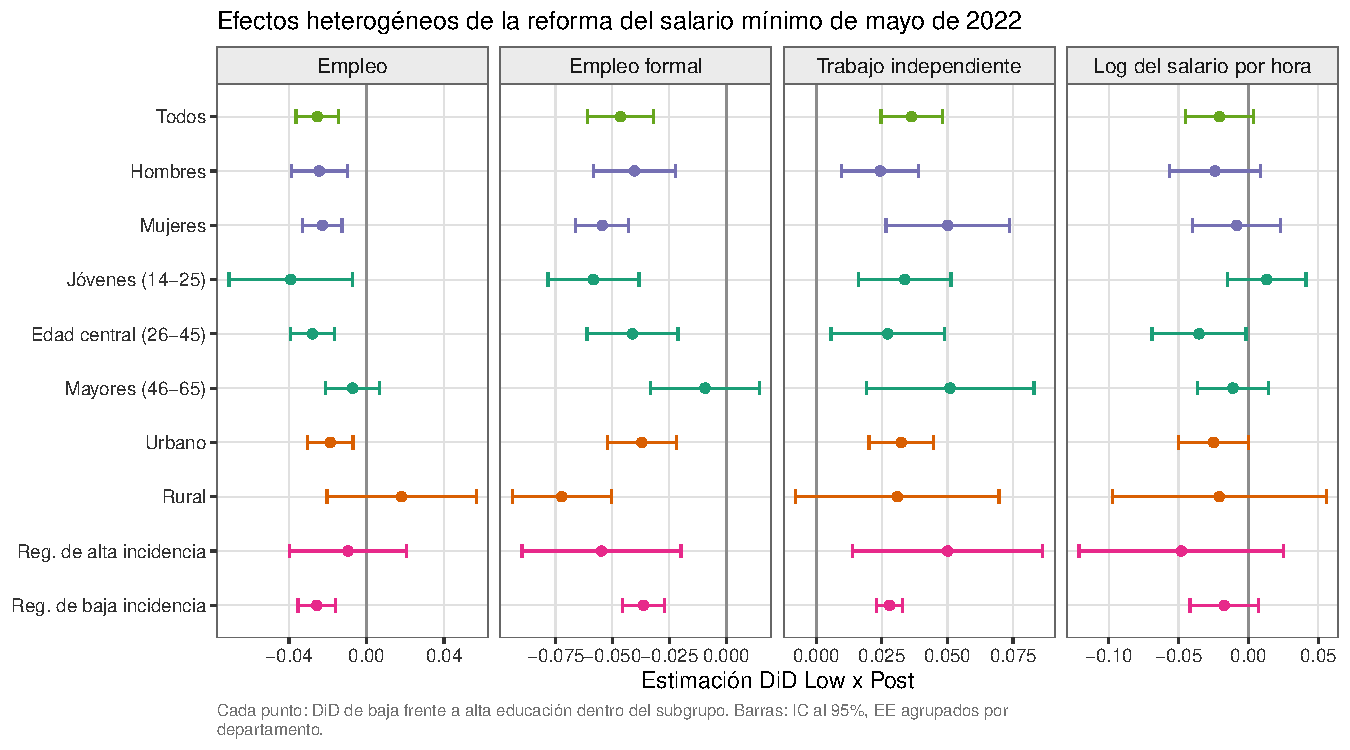
\includegraphics[width=0.98\textwidth]{fig6_heterogeneity.pdf}
\caption{Efectos heterogéneos de la reforma de 2022. Cada punto es la estimación de
diferencias en diferencias $\mathrm{Low}\times\mathrm{Post}$ dentro del subgrupo indicado,
con intervalos de confianza al noventa y cinco por ciento basados en errores estándar
agrupados por departamento.}
\label{fig:het}
\end{figure}

\subsection{Márgenes de ajuste}

¿Dónde ocurre exactamente la reasignación? Cuatro márgenes orientados a los mecanismos
precisan el panorama (Cuadro~\ref{tab:margins} del Apéndice). Primero, la proporción de
asalariados de baja educación empleados \emph{sin contrato escrito} aumenta en 3.1 puntos
porcentuales respecto de los asalariados de alta educación, de modo que la informalización
opera dentro del empleo asalariado y no solo mediante salidas hacia el trabajo
independiente.\footnote{La pregunta sobre el contrato se eliminó del cuestionario reducido
que se aplicó en quince regiones en febrero de 2021; codifico esas observaciones como
faltantes y no como carentes de contrato, lo que importa para este margen.} Segundo, el
empleo se recompone hacia las \emph{microunidades}: la probabilidad de que un trabajador de
baja educación esté empleado en un establecimiento de a lo sumo veinte trabajadores
aumenta en 2.8 puntos, y las unidades pequeñas son precisamente donde la fiscalización es
más escasa. Tercero, según la descomposición del empleo informal del INEI (disponible hasta
2023), el margen desplazado recae en el \emph{sector informal} propiamente dicho (+2.4
puntos) y no en empleos no registrados dentro de empresas formales (+0.8, no
significativo): los trabajadores no se quedaron con empleadores formales de manera
irregular, sino que se trasladaron a unidades productivas informales. Cuarto, la
proporción de asalariados con menos de un año de antigüedad no se mueve, de modo que el
ajuste no se manifiesta como un congelamiento de contrataciones entre quienes siguen siendo
asalariados.

Dos divisiones adicionales por subgrupo ubican la carga. Los efectos de composición se
concentran casi por completo entre los \emph{no jefes} de hogar (perceptores secundarios de
ingreso, cuya formalidad cae 6.8 puntos, frente a un efecto nulo para los jefes de hogar) y
entre los trabajadores no indígenas, lo que es coherente con los mercados laborales urbanos
de la costa, donde se concentra el empleo formal en torno al piso. En suma, los empleos
formales marginales que se disolvieron fueron los de perceptores secundarios en pequeñas
empresas urbanas.

\subsection{Efectos salariales distributivos}

La ausencia de un efecto salarial promedio podría, en principio, ocultar movimientos que se
compensan en distintos puntos de la distribución salarial, dado que se espera que un
salario mínimo comprima la cola inferior. Para examinarlo, estimo regresiones por cuantiles
incondicionales (función de influencia recentrada) a la manera de
\citet{firpo_fortin_lemieux_2009}, aplicando la especificación de diferencias en
diferencias a la función de influencia de cada decil del logaritmo del salario real por
hora. La Figura~\ref{fig:rif} grafica el coeficiente $\mathrm{Low}\times\mathrm{Post}$ a lo
largo de los deciles. Las estimaciones son no positivas en todos los deciles, en su mayoría
entre $-2$ y $-4$ por ciento y significativas en algunos deciles intermedios; lo crucial es
que no hay ningún efecto positivo en los deciles inferiores, donde un salario mínimo
vinculante y fiscalizado comprimiría la distribución desde abajo. La evidencia distributiva
refuerza, por lo tanto, la ausencia de respuesta en las remuneraciones: la reforma no elevó
la cola inferior de la distribución salarial de los poco calificados respecto de la de los
calificados. Esto es coherente con la distribución de ingresos de la Figura~\ref{fig:dist},
que muestra poco movimiento hacia el nuevo piso, y con la interpretación de que, en un
mercado laboral con incumplimiento generalizado, el mínimo legal no fue vinculante para la
mayoría de los trabajadores poco calificados.

\begin{figure}[!t]
\centering
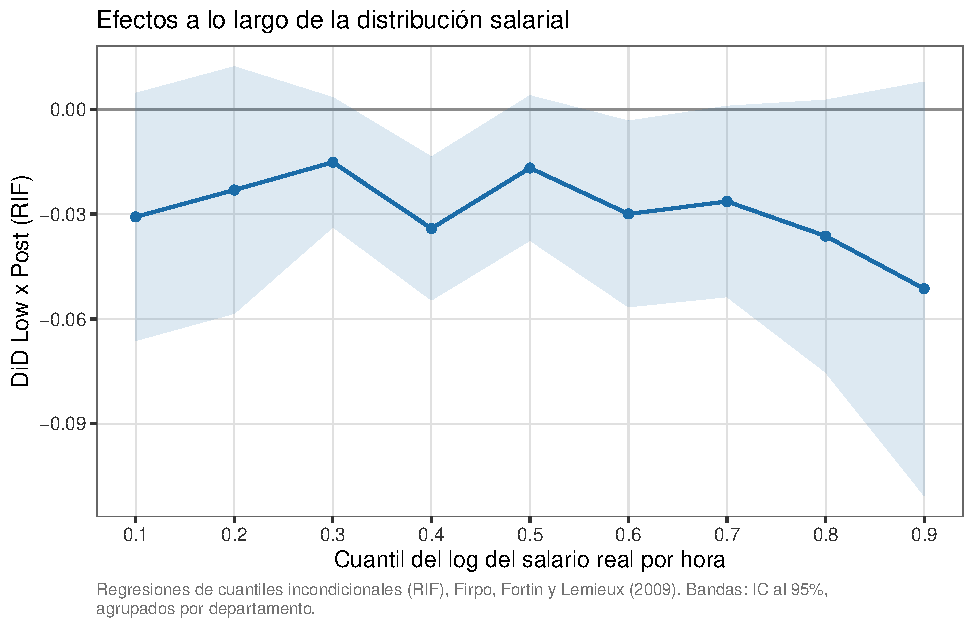
\includegraphics[width=0.72\textwidth]{fig8_rif_quantile.pdf}
\caption{Efectos salariales distributivos. Cada punto es el coeficiente de diferencias en
diferencias $\mathrm{Low}\times\mathrm{Post}$ de una regresión por cuantiles
incondicionales (RIF) en el decil indicado del logaritmo del salario real por hora
\citep{firpo_fortin_lemieux_2009}. Las bandas son intervalos de confianza al noventa y
cinco por ciento con errores agrupados por departamento.}
\label{fig:rif}
\end{figure}

\section{Discusión}\label{sec:discussion}

\subsection{Mecanismos}

La evidencia describe un salario mínimo que movió trabajadores y no salarios. La reasignación es mi resultado más robusto: la formalidad cae y el trabajo independiente aumenta, los desplazamientos crecen con la incidencia (\emph{bite}) regional del piso y los confirma un diseño de exposición continua con inferencia por aleatorización. El mecanismo natural es el clásico: un piso que se vuelve vinculante en el sector cubierto induce una reasignación hacia el sector no cubierto, el canal de desplazamiento que \citet{jaramillo_lopez_2006} documentan para el Perú y \citet{ham_2018_honduras} para Honduras. Su incidencia aparece exactamente donde ese mecanismo lo predice: entre los jóvenes, entre las mujeres y en los departamentos de alta incidencia, es decir, en los trabajadores y lugares donde el nuevo piso cortó más hondo en la distribución salarial. Las transiciones de panel de la Sección~\ref{sec:transitions} identifican el flujo detrás del cambio en el stock y precisan el mecanismo en un aspecto importante: la retención de los trabajadores formales en su puesto no cayó, mientras que la entrada a empleos formales desde la informalidad se redujo casi a la mitad, de modo que la reasignación operó a través de la creación de vínculos formales y no de su destrucción. El piso no expulsó a quienes ya estaban empleados; le cerró la puerta a nuevos vínculos formales para los trabajadores de baja educación. Es el mismo ajuste por el margen de las contrataciones que \citet{dustmann_2022} documentan para Alemania, y explica por qué el costo recae en los entrantes marginales, los perceptores secundarios de ingreso, los jóvenes y las mujeres, y no en los trabajadores protegidos que ya tenían un puesto. El aumento simultáneo de las horas es coherente con el paso hacia el trabajo independiente, donde las horas están menos restringidas. Un matiz acota el destino del margen desplazado: en el diseño regional, la tasa incondicional de trabajo independiente no aumenta con la exposición (Cuadro~\ref{tab:uncond} del apéndice), de modo que entre departamentos el margen absoluto robusto es la destrucción de empleo formal, y el aumento de la participación del trabajo independiente en el empleo refleja en parte la reducción de la base de empleo; el desplazamiento absoluto hacia el trabajo por cuenta propia aparece en el contraste por educación, donde se compara directamente a los trabajadores desplazados con sus sustitutos más cercanos.

¿Por qué la reasignación no estuvo acompañada de una respuesta salarial agregada? No porque el piso sea letra muerta: la evidencia de primera etapa muestra que, dentro del sector formal, el pico en el mínimo antiguo migró casi por completo al nuevo, de modo que los empleadores cubiertos cumplieron. La explicación está en la aritmética de la cobertura en un mercado laboral con dos sectores \citep{ulyssea_2018}. Solo el 13 por ciento de los trabajadores poco calificados ocupados es formal, así que incluso el cumplimiento pleno dentro del segmento formal mueve muy poco el salario promedio del grupo; mientras tanto, la remuneración en el segmento informal se alejó \emph{aún más} por debajo del piso, y ambas respuestas se compensan en el agregado. La inflación agrava el cuadro: el aumento de 2022, de diez por ciento en términos nominales, coincidió con una inflación de precios al consumidor de alrededor de ocho por ciento, de modo que el valor real del piso apenas subió y luego se erosionó. Un piso que solo se respeta donde los costos laborales son fiscalizables no puede elevar la distribución salarial del grupo, pero sí puede influir en los arreglos de empleo que eligen empresas y trabajadores, y según mis estimaciones lo hizo. Es la misma lógica de reasignación que \citet{dustmann_2022} documentan entre establecimientos en Alemania, trasladada al margen que importa en una economía en desarrollo: la frontera entre el trabajo formal y el informal \citep{jales_2018}.

Dos salvedades acotan esta lectura. La reasignación, aunque robusta a la especificación y a la inferencia basada en el diseño, es sensible a violaciones moderadas de las tendencias paralelas en el contraste por educación \citep{rambachan_roth_2023}, y no reaparece en torno a la reforma de 2025, donde el mismo diseño y las mismas magnitudes arrojan efectos nulos en todos los márgenes y una pequeña estimación de signo opuesto para el trabajo independiente. Interpreto el contraste entre ambos episodios como dependencia del estado, y la Sección~\ref{sec:reconciliation} examina directamente las dos variables de estado candidatas: la evidencia favorece la posición del piso en la distribución de la remuneración formal (el aumento de 2022 barrió una franja que concentraba la cuarta parte de la remuneración formal de baja educación, mientras que el de 2025 barrió una más delgada) y rechaza la versión basada en la rotación del mercado laboral, pues la creación de vínculos formales era de hecho mayor en vísperas de 2025. La evidencia del margen de entrada de la Sección~\ref{sec:transitions} identifica el margen por el que debe operar cualquier dependencia del estado de este tipo: la creación de nuevos vínculos formales, cuya rentabilidad gobierna el piso. Sin embargo, no puedo descartar del todo la lectura alternativa, según la cual una dinámica residual de recuperación correlacionada con la educación contribuye a las estimaciones de composición de 2022; lo que me inclina hacia una interpretación causal es la evidencia de dosis-respuesta y de exposición continua, pues una recuperación diferenciada por educación no tiene por qué seguir el índice de Kaitz regional previo a la reforma.

\subsection{Conciliación con la literatura previa}\label{sec:reconciliation}

Mis resultados encajan bien con parte de la evidencia previa y entran en tensión con el resto, y ese patrón es informativo en sí mismo. Hacen eco del trabajo peruano anterior de \citet{jaramillo_lopez_2006}, quienes encontraron que la reforma de 2003 fue en gran medida inocua, con desplazamiento hacia la informalidad, y de \citet{cespedes_2005}, quien encontró efectos concentrados entre los jóvenes. Son coherentes con el hallazgo internacional general de que los aumentos del salario mínimo en este rango producen efectos pequeños sobre el empleo \citep{card_krueger_1995, cengiz_2019}.

La tensión es con el estudio peruano más reciente. \citet{jimenez_2023} encuentra que la reforma de 2016 elevó los salarios formales entre cuatro y cinco por ciento y aumentó la formalidad, un patrón de efecto faro que no reproduzco para 2022. Tres diferencias explican plausiblemente la divergencia. El aumento de 2016 ocurrió en un periodo de baja inflación, por lo que su incidencia real fue mayor y más duradera que la del aumento de 2022, erosionado por la inflación. La identificación difiere: \citet{jimenez_2023} usa una dosis a nivel departamental definida sobre la distribución salarial formal, mientras que yo contrasto a trabajadores de baja y alta educación a nivel individual, un diseño que da más peso al amplio segmento informal de los poco calificados. Y el contexto macroeconómico difiere: crecimiento estable en 2016 frente a una recuperación pospandemia en 2022. Una observación ayuda a discriminar entre estas explicaciones: 2016, el episodio con efecto faro, fue también un año tranquilo, al igual que 2025, en el que no encuentro efecto alguno, de modo que el estado macroeconómico por sí solo no puede explicarlo todo. Lo que separa a 2016 de 2025 es el \emph{nivel} del piso cuando llegó el aumento: en 2016 el mínimo estaba bastante por debajo del salario mediano y un aumento real podía plausiblemente propagarse como norma, mientras que hacia 2025 el piso ya superaba la mediana nacional, de modo que un nuevo aumento partía de un nivel que la práctica ya había dejado de respetar para el trabajador marginal. Bajo esta lectura, los tres episodios se ordenan según dos variables de estado: cuán alto se ubica ya el piso en la distribución salarial y cuánta reasignación está atravesando el mercado laboral. Un piso moderado que sube en un mercado estable puede elevar las normas (2016); un piso alto que sube en medio de la reasignación pospandemia mueve el margen de composición (2022); y un piso alto que sube en un mercado asentado no mueve nada (2025).

Como una historia con dos variables de estado libres puede racionalizar casi cualquier cosa, examino ambas directamente y dejo que los datos descarten una. La variable de posición del piso se comporta como la historia exige: en vísperas de la reforma de 2022, el 24 por ciento de los asalariados formales de baja educación ganaba dentro de la franja que el nuevo piso estaba por barrer y el 16 por ciento se acumulaba en el piso antiguo, mientras que en vísperas de la reforma de 2025 esas proporciones habían bajado a 17 y 14 por ciento. La variable de reasignación no: la proporción de nuevas contrataciones entre los trabajadores formales de baja educación era \emph{mayor} en 2024 (41 por ciento) que antes de la reforma de 2022 (32 por ciento), de modo que el resultado nulo de 2025 no puede atribuirse a una escasez de nuevos vínculos formales. Una prueba de dosis a nivel departamental apunta en la misma dirección: interactuar el contraste por educación con la creación de vínculos formales previa a la reforma no produce ningún gradiente en ninguno de los dos episodios, con o sin el control de Kaitz.\footnote{Los momentos de las variables de estado y las estimaciones de dosis se incluyen en el paquete de replicación (\texttt{state\_premise.csv}, \texttt{state\_dose.csv}).} Por ello descarto la versión del argumento basada en la rotación y apoyo la interpretación en la posición del piso: el margen de entrada se cierra cuando el nuevo piso barre una franja densa de la remuneración formal, como en 2022, y le queda poco por cerrar cuando el piso ya superó el rango que la práctica de remuneración formal respeta, como en 2025. El contraste en la franja barrida es real pero modesto, por lo que presento esta interpretación como la más coherente con la evidencia y no como un hecho establecido.

\subsection{Validez externa y limitaciones}

Cinco limitaciones acotan la interpretación. Primero, la identificación descansa en el supuesto de que, sin la reforma, los trabajadores de baja y alta educación habrían seguido trayectorias paralelas. Pongo a prueba este supuesto donde es posible y acoto las consecuencias de que no se cumpla; las tendencias previas de la formalidad son planas, pero la prueba de tendencias previas salariales rechaza debido a un único trimestre de inicios de 2021, y la serie de empleo muestra una clara tendencia previa de recuperación, razón por la cual formulo la conclusión salarial como ``ninguna ganancia detectable'' y no como un nulo preciso, y trato el resultado sobre el nivel de empleo como no concluyente. Segundo, el diseño identifica efectos sobre los trabajadores poco calificados en relación con los calificados. El grupo de comparación no está del todo libre de exposición (el 40 por ciento de los asalariados calificados ganaba por debajo del nuevo piso antes de la reforma), de modo que las estimaciones son magnitudes relativas que, en primer orden, subestiman el efecto sobre los plenamente expuestos; el diseño de exposición continua aborda en parte este problema al prescindir del grupo de comparación. Tercero, el diseño principal usa cortes transversales repetidos; el análisis con el Panel ENAHO de la Sección~\ref{sec:transitions} aborda directamente la distinción entre flujos y stocks, pero es anual y no trimestral, su referencia previa a la reforma incluye transiciones desde el año pandémico 2020 y sus muestras de base formal son modestas, por lo que lo trato como una corroboración del mecanismo y no como fuente de magnitudes precisas. Cuarto, la informalidad en 2024 se mide con un indicador reconstruido y no con el oficial; dentro de la ventana de validación de 2025 el indicador se reconstruye de manera consistente en todos los trimestres, pero el empalme de 2024 añade error de medición al tramo final del estudio de eventos de 2022. Finalmente, la ventana abarca como máximo diez trimestres limpios posteriores a la reforma, por lo que me refiero a efectos de corto y mediano plazo y no al ajuste de largo plazo del capital ni a la entrada y salida de empresas.

\subsection{Implicancias de política}

Los resultados dejan un mensaje sobrio para la política de salario mínimo en una economía de alta informalidad. Un piso que no se hace cumplir para la mayoría de sus beneficiarios previstos hace poco por elevar su remuneración, y donde sí es vinculante, en el sector formal, puede empujar a algunos trabajadores hacia arreglos menos protegidos. Elevar el salario mínimo es, por tanto, un instrumento imperfecto para aumentar los ingresos de los poco calificados en el Perú, conclusión que hace eco de \citet{jaramillo_lopez_2006}. Esto no significa que el salario mínimo sea inocuo ni inútil; mis estimaciones son relativas y mi ventana es corta. Pero sí implica que la formalización y la fiscalización son condiciones previas para que el piso llegue a los trabajadores que busca proteger. Sin ellas, el margen de ajuste es la composición del empleo y no el nivel de la remuneración.

\section{Conclusiones}\label{sec:conclusion}

He estudiado cómo el aumento del salario mínimo peruano de 2022, de 930 a 1025 soles, afectó a trabajadores con distintos niveles educativos, usando datos trimestrales de la ENAHO y un diseño de diferencias en diferencias que aprovecha la exposición marcadamente distinta de los trabajadores de baja y alta educación a una única reforma nacional. Mi hallazgo central es que la reforma desplazó la composición del empleo poco calificado y no el nivel de su remuneración: el empleo formal cayó 4.6 puntos porcentuales, una quinta parte de su nivel de base, y el trabajo independiente aumentó 3.6 puntos, con tendencias previas de la formalidad que superan su prueba conjunta y una deriva residual que cuantifico y corrijo, desplazamientos mayores donde el piso cortó más hondo en la distribución salarial regional y la confirmación de un diseño de exposición continua con inferencia por aleatorización. Los datos de panel enlazados ubican el margen: los trabajadores formales en su puesto fueron retenidos, mientras que la entrada a empleos formales de los trabajadores de baja educación cayó casi a la mitad, de modo que el piso operó cerrando la puerta a nuevos vínculos formales y no disolviendo los existentes. Ninguna respuesta salarial acompañó el desplazamiento: los salarios relativos de los trabajadores de baja educación no subieron ni en la media ni en ningún punto de la distribución, y la proporción de asalariados que gana por debajo del piso no cayó, lo que señala el incumplimiento como la razón por la que el piso no pudo elevar la remuneración. El efecto sobre el empleo total no puede precisarse y se confunde con la recuperación pospandemia desigual. En torno a la reforma de enero de 2025, de igual magnitud, ni los salarios ni la composición respondieron. Examinar directamente el contraste favorece una lectura basada en la posición del piso frente a una basada en la rotación del mercado laboral: el aumento de 2022 barrió una franja que concentraba la cuarta parte de la remuneración formal de baja educación, mientras que el de 2025 barrió una franja más delgada en una distribución que el piso ya había rebasado, aun cuando la creación de vínculos formales era, si acaso, mayor en 2024. El margen de reasignación opera cuando el nuevo piso atraviesa el rango donde efectivamente se ubica la remuneración formal, y queda inactivo cuando ya lo ha superado.

La lectura más económica de estos resultados es que, en un mercado laboral donde la informalidad es generalizada y la fiscalización débil, un aumento moderado del mínimo legal, erosionado por la inflación, no eleva la remuneración de los poco calificados; lo que mueve, cuando mueve algo, es la asignación de los trabajadores entre arreglos formales e informales. Esto matiza la visión del efecto faro del salario mínimo peruano que surge de los estudios de reformas anteriores y apunta al margen informal como el canal central de ajuste.

De aquí se desprenden dos líneas de investigación futura. La primera es afinar la evidencia sobre transiciones con datos enlazados de mayor frecuencia, ya sea la EPEN mensual o los registros administrativos de la Planilla Electrónica, que permitirían fechar dentro del año la respuesta por el margen de las contrataciones y seguir a las mismas empresas y trabajadores a lo largo de ambas reformas; mi panel anual establece el margen, pero no su dinámica fina. La segunda es estudiar directamente la interacción entre la política de salario mínimo y la fiscalización, pues mis resultados sugieren que los réditos de elevar el piso dependen de que este pueda hacerse vinculante. A medida que se acumulen más trimestres posteriores a la reforma, también será posible rastrear el ajuste de largo plazo que una ventana corta como la mía no logra capturar.


\newpage
\bibliography{paper/references}

\newpage
\appendix
\section{Apéndice de datos}\label{app:data}

\subsection{Muestra y construcción de variables}

Agrupo los veinte módulos trimestrales de empleo de la ENAHO (módulo 500) para 2021Q1--2025Q4; el análisis principal usa 2021Q1--2024Q4 y la validación usa 2024Q1--2025Q4. La muestra en edad de trabajar comprende a las personas de 14 a 65 años con información de educación. Todas las estadísticas usan el factor de expansión de empleo del módulo (\texttt{fac500a}). Este factor está calibrado para que el año completo de entrevistas se expanda a la proyección anual de población; cada submuestra trimestral se expande, por tanto, a aproximadamente la cuarta parte de la población, lo que es irrelevante para las medias, proporciones y estimaciones de regresión ponderadas que uso a lo largo del trabajo (numerador y denominador se escalan juntos) y solo importaría para totales poblacionales, que nunca estimo. La partición trimestral sigue el mes de la entrevista y coincide con el diseño de la propia encuesta: la inferencia nacional trimestral es un nivel de inferencia oficial de la ENAHO en las fichas técnicas tanto de 2021 como de 2025, y la muestra no panel vuelve a visitar los mismos conglomerados en los mismos meses cada año. Verifico ambas propiedades en los microdatos para toda la ventana: los 5359 conglomerados aparecen en todos los años de 2021 a 2025, la superposición de unidades primarias de muestreo entre el mismo trimestre de años consecutivos va de 70 a 92 por ciento (frente a 2 a 5 por ciento entre trimestres distintos), y cada trimestre es una réplica internamente balanceada del diseño. Conviene registrar dos cambios en la encuesta durante la ventana. Primero, la modalidad mixta de entrevista adoptada durante la pandemia (prioridad a la entrevista presencial, con seguimiento telefónico para los miembros ausentes) siguió siendo el estándar hasta 2025, de modo que la modalidad es en líneas generales consistente en mi periodo de estudio; la única excepción es febrero de 2021, cuando un cuestionario telefónico reducido en quince regiones omitió, entre otras preguntas, la del tipo de contrato (faltante para la mitad de los asalariados de ese mes), lo que no afecta a ninguno de los resultados de base (la informalidad de 2021 proviene del indicador oficial del INEI y las preguntas de ingreso se mantuvieron) y se trata explícitamente en el único margen del apéndice que usa contratos. Segundo, la ficha técnica de 2025 describe el diseño como bietápico, con conglomerados urbanos de unas 140 viviendas, frente a la descripción polietápica de 2021; los identificadores y conteos de conglomerados son, no obstante, continuos a lo largo de la ventana, de modo que se trata de una reformulación de la documentación y no de un quiebre en la muestra. Los departamentos son las 25 unidades administrativas de primer nivel derivadas de los dos primeros dígitos del \texttt{ubigeo}; el indicador urbano se deriva del estrato de muestreo.

\paragraph{Educación y grupos de calificación.} El nivel educativo alcanzado corresponde a la variable \texttt{p301a} de la ENAHO. Verifiqué su codificación con la distribución ponderada del nivel alcanzado. Los trabajadores poco calificados son aquellos con \texttt{p301a} entre 1 y 6 (desde sin nivel hasta secundaria completa); los trabajadores calificados son aquellos con \texttt{p301a} entre 7 y 11 (desde superior no universitaria hasta posgrado). Se excluyen la educación básica especial (código 12) y los valores faltantes.

\paragraph{Ingreso laboral y salarios.} La ENAHO registra la remuneración de los asalariados por periodo de pago: \texttt{p524a1} es el pago bruto, incluidas las horas extra, y \texttt{p523} su frecuencia (diaria, semanal, quincenal o mensual). El cincuenta y cuatro por ciento de los asalariados de baja educación recibe pagos con frecuencia no mensual, frente al quince por ciento de los asalariados de alta educación, por lo que convierto todos los pagos a equivalentes mensuales con los mismos factores implícitos en la variable de ingreso anualizado del propio INEI (\texttt{i524a1}): 25 para la frecuencia diaria, $52/12$ para la semanal, 2 para la quincenal y 1 para la mensual. La distribución ponderada completa de frecuencias entre los asalariados privados con ingresos válidos es de 2 por ciento diaria, 45 semanal, 9 quincenal y 45 mensual para el grupo de baja educación, frente a 1, 18, 6 y 76 por ciento para el grupo de alta educación; la variable de frecuencia nunca falta en esa muestra. Los asalariados comprenden a empleados y trabajadores del hogar (\texttt{p507} en $\{3,4,6\}$); los trabajadores del hogar tienen derecho al salario mínimo desde la Ley 31047. Para los empleadores y los trabajadores por cuenta propia, el ingreso laboral es la ganancia neta (\texttt{p530a}), que ya es mensual. Como el ingreso reportado se refiere al mes anterior a la entrevista, deflacto en ese mes de referencia (las entrevistas de enero se remontan a diciembre del año anterior) con el índice de precios al consumidor de Lima con base diciembre de 2021, y evalúo el mínimo legal vigente en ese mismo mes de referencia al clasificar a los trabajadores como remunerados por debajo del piso. El salario real por hora divide el ingreso laboral mensual equivalente entre $4.345$ veces las horas semanales en la ocupación principal (\texttt{p513t}; la variable de horas imputadas del INEI, \texttt{i513t}, la reemplaza cuando \texttt{p513t} falta, pero ninguna observación de la muestra de análisis salarial y menos del 0.01 por ciento de la muestra de horas lo requieren). Los resultados salariales excluyen a los trabajadores del sector público, cuya remuneración se fija mediante escalas propias, y se winsorizan una sola vez en los percentiles 0.5 y 99.5 de la muestra agrupada de asalariados privados.

\paragraph{Informalidad.} El indicador oficial de empleo informal del INEI (\texttt{ocupinf}, codificado como 1 para informal y 2 para formal en estos archivos) está disponible para 2021--2023 pero no para 2024--2025. Reconstruyo un indicador consistente a partir de variables primitivas disponibles en todos los años. Un empleado asalariado o trabajador del hogar se clasifica como formal si está afiliado a un sistema de pensiones (\texttt{p558a1}--\texttt{p558a4}, cuyas opciones seleccionadas se marcan con su código de opción y no con unos) o si tiene un contrato laboral formal (\texttt{p511a} entre 1 y 6); un empleador o trabajador por cuenta propia se clasifica como formal si la unidad productiva está registrada (\texttt{p510a1}); los trabajadores familiares no remunerados son siempre informales. Validada contra \texttt{ocupinf} en los años de superposición 2021--2023, esta regla coincide con la clasificación oficial para el 87.8 por ciento de los ocupados y arroja una tasa de informalidad de 74.9 por ciento, frente al 79.1 por ciento oficial. Uso el indicador oficial siempre que está disponible y la reconstrucción solo para 2024--2025; dentro de la ventana de validación 2024--2025 el indicador se reconstruye en todos los trimestres, de modo que allí se mide de manera consistente.

\paragraph{Salario mínimo e incidencia.} El calendario del salario mínimo legal se toma de los decretos y se verifica con la serie del Banco Central de Reserva del Perú (PN02124PM); el deflactor del IPC es la serie PN38705PM del BCRP (Lima, diciembre de 2021 $=$ 100), y ambos insumos se regeneran con un script documentado en el paquete de replicación. El índice de Kaitz departamental es el cociente entre el mínimo posterior a la reforma (1025 soles) y el salario mensual equivalente mediano ponderado de los asalariados privados del departamento antes de la reforma (2021Q1--2022Q1). La medida de fracción afectada es la proporción ponderada, antes de la reforma, de asalariados privados que ganaban menos de 1025 soles.

\paragraph{El Panel ENAHO.} El análisis de transiciones de la Sección~\ref{sec:transitions} usa el Panel ENAHO 2020--2024 (encuesta 978 del INEI, publicada en noviembre de 2025), cuyo módulo de empleo (\texttt{enaho01a-2020-2024-500-panel.dta}) contiene un registro por persona con variables con sufijo de año para 2020 a 2024. Las personas observadas en ambos años de un par se identifican con los indicadores \texttt{perpanel} (23\,983 personas enlazadas para 2021--22 y 23\,245 para 2022--23) y se ponderan con los factores de expansión de panel del INEI, \texttt{facpanel}, que corrigen por desgaste y no respuesta; la inferencia oficial para pares de años consecutivos es nacional, urbana y rural, y por región natural. Los estados de empleo replican exactamente las definiciones de corte transversal: ocupado es \texttt{ocu500}${}=1$; el estado formal privado requiere empleo en el sector privado con un puesto formal; la informalidad usa el \texttt{ocupinf} oficial donde se publica y, en los demás casos, la reconstrucción con la Regla F descrita arriba; el trabajo independiente comprende a los trabajadores por cuenta propia y a los empleadores. La educación en el año base define los grupos de calificación. Como el panel es anual y la reforma entró en vigor el 1 de mayo de 2022, las observaciones de cada par se clasifican según el mes de entrevista de 2022, como se describe en las notas del Cuadro~\ref{tab:transitions}.

\paragraph{Intensidad de las protestas.} La intensidad departamental de la crisis política de 2022--23 se mide a partir de los reportes mensuales de conflictos de la Presidencia del Consejo de Ministros (Secretar\'ia de Gesti\'on Social y Di\'alogo, ``Reporte de Conflictos Sociales''), cuyos cuadros de seguimiento de la crisis registran el número máximo de personas movilizadas en acciones de protesta en cada departamento, por semana y por mes. Tomo el máximo de cada departamento en los reportes de enero y febrero de 2023, los dos meses en que la movilización nacional alcanzó su punto más alto (el reporte de diciembre de 2022 es anterior al cuadro), lo divido entre la población en edad de trabajar del departamento (cuatro veces la suma trimestral media de los factores de expansión de la ENAHO) y estandarizo el resultado entre los 25 departamentos. El cuadro transcrito y los documentos fuente se incluyen en el paquete de replicación.

\subsection{Resultados complementarios}

El Cuadro~\ref{tab:ddd} presenta las estimaciones de triple diferencia y el Cuadro~\ref{tab:loo} los rangos de estabilidad excluyendo un departamento a la vez discutidos en la Sección~\ref{sec:robustness}; los Cuadros~\ref{tab:expocells}--\ref{tab:margins} reúnen los diagnósticos del diseño de exposición, las verificaciones sectoriales y ocupacionales, las cotas de selección y los cálculos de potencia, los resultados de diferencias en diferencias sintéticas y de potencia de la prueba previa, y los márgenes de ajuste. El Cuadro~\ref{tab:crisis} presenta la robustez del diseño de exposición regional continua frente a la crisis política y el Cuadro~\ref{tab:uncond} los resultados de composición incondicionales, ambos discutidos en la Sección~\ref{sec:robustness}. El Cuadro~\ref{tab:placebo} presenta las reformas placebo en el tiempo y confirma que los placebos salariales son nulos, mientras que los placebos de empleo están contaminados por la tendencia previa de la pandemia. Las estimaciones doblemente robustas de \citet{santanna_zhao_2020} aparecen junto a las estimaciones con efectos fijos bidireccionales en el Cuadro~\ref{tab:main}. El Figura~\ref{fig:val2025} muestra el estudio de eventos en torno a la reforma de enero de 2025 usado en la validación fuera de muestra.

\input{../../tables/es/tab_triplediff}

\input{../../tables/es/tab_leaveoneout}

\input{../../tables/es/tab_exposure}

\input{../../tables/es/tab_sector_occ}

\input{../../tables/es/tab_lee_mde}

\input{../../tables/es/tab_sdid_power}

\input{../../tables/es/tab_margins}

\input{../../tables/es/tab_migration}

\input{../../tables/es/tab_crisis}

\input{../../tables/es/tab_uncond}

\paragraph{Deflactores.} Todas las regresiones salariales incluyen efectos fijos de trimestre, que absorben la inflación nacional, de modo que las estimaciones de diferencias en diferencias del logaritmo del salario no dependen del deflactor nacional; y las medidas de incidencia comparan salarios nominales con el piso legal nominal, por lo que no involucran deflactación alguna. Una deflactación de precios específica por departamento solo importaría para comparaciones entre departamentos de \emph{niveles} de salario real, que no cumplen ningún papel en la identificación.

\begin{figure}[!t]
\centering
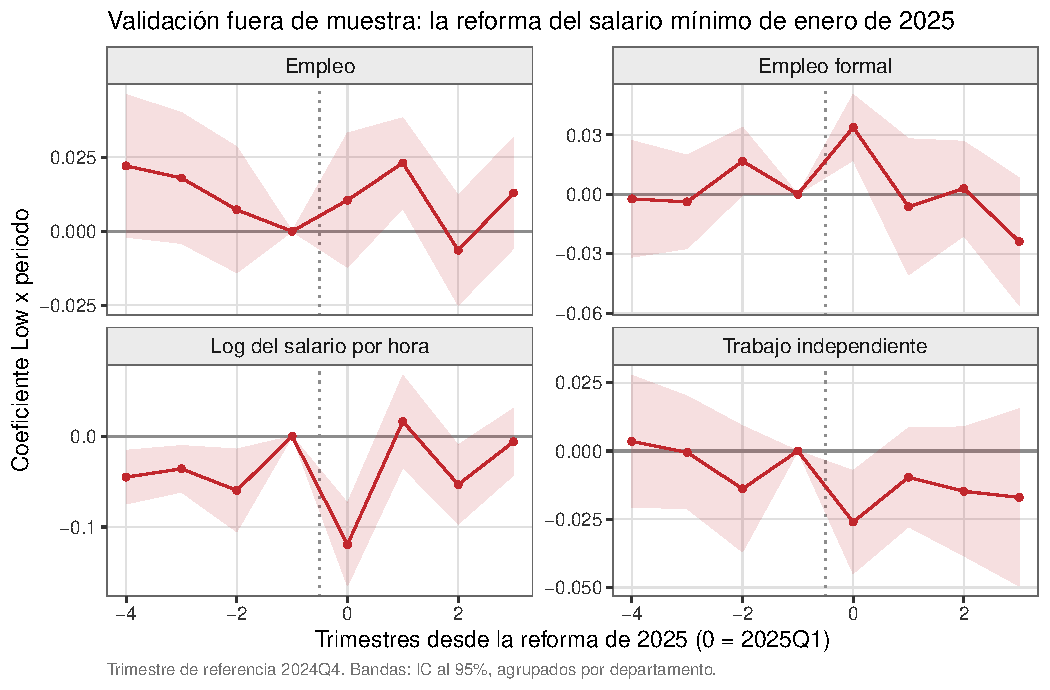
\includegraphics[width=0.9\textwidth]{fig9_validation2025.pdf}
\caption{Estudio de eventos en torno a la reforma de enero de 2025 (validación fuera de muestra). Coeficientes de la interacción del indicador de baja calificación con indicadores de trimestre; trimestre de referencia 2024Q4. Las bandas son intervalos de confianza al noventa y cinco por ciento con errores agrupados por departamento.}
\label{fig:val2025}
\end{figure}

\begin{table}[!tbp]\centering
\caption{Reformas placebo en el tiempo (solo ventana previa a la reforma)}\label{tab:placebo}
\begin{threeparttable}
\input{../../tables/es/tab_placebo_body}
\begin{tablenotes}\footnotesize
\item Notas: Cada celda es el coeficiente $\mathrm{Low}\times\mathrm{Post}$ de una estimación placebo de diferencias en diferencias que asigna una reforma ficticia al trimestre indicado, estimada usando solo datos previos a la reforma (2021Q1--2022Q1). Errores estándar agrupados por departamento entre paréntesis; todas las estimaciones se ponderan con los factores de expansión de la ENAHO. $^{*}p<0.1$, $^{**}p<0.05$, $^{***}p<0.01$.
\end{tablenotes}
\end{threeparttable}
\end{table}


\end{document}
